\chapter{Two-Dimensional Potential Flows}
\begin{equation}
\left.
\begin{aligned}
\text{Incompressible}&\colon\nabla\cdot\mathbf{v} = 0\\
\text{Irrotational}&\colon\nabla\times\mathbf{v} = 0
\end{aligned}
\right\}
\Longrightarrow\nabla^2\Phi = 0
\label{eq: 5-0-1}
\end{equation}
Equation \eqref{eq: 5-0-1} can be solved via using Complex-Variable Theory. 
\section{Brief Review of Complex Theory}
\begin{itemize}
\item A complex variable: $z = x+iy = re^{i\theta}$, $i= \sqrt{-1}$, $r=\sqrt{x^2 + y^2}$, $\theta = \arctan(y/x)$
\item A complex function
\[
f(z) = \xi(x,y) + i\eta(x,y)
\]
\begin{align*}
\xi\equiv\Re\left\{f\right\}, &&\eta\equiv\Im\left\{f\right\}
\end{align*}
\item Complex conjugate (C-C)
\begin{align*}
\bar{z} = x-iy, && z,\bar{z}\colon\text{C-C pair}
\end{align*}
\[
\overline{f(z)}\colon\text{C-C of }f(z)
\]
Note that $\overline{f(z)}\neq\bar{f}(z)\neq f(\bar{z})$, e.g.\\
if $f(z) = \left(2+3i\right)z+e^{4iz}$, $\overline{f(z)} = \left(2-3i\right)\bar{z}+e^{-4i\bar{z}}$,$\bar{f}(z) = \left(2-3i\right)z + e^{-4iz}$, $f(\bar{z}) = \left(2+3i\right)\bar{z} + e^{4i\bar{z}}$
\item The conjugate $z$ and $\bar{z}$
\[
\text{Since }
\left\{
\begin{aligned}
z &= x+iy \\
\bar{z} &= x-iy
\end{aligned}
\right.
\Longrightarrow
\left\{
\begin{aligned}
x &= \frac{1}{2}\left(z+\bar{z}\right) \\
y &= -\frac{i}{2}\left(z-\bar{z}\right)
\end{aligned}
\right.
\]
\[
(x,y)\Longleftrightarrow (z,\bar{z})
\]
\[
\left\{
\begin{aligned}
\frac{\partial}{\partial z} 
&= \frac{\partial x}{\partial z}\frac{\partial}{\partial x} + \frac{\partial y}{\partial z}\frac{\partial}{\partial y} = \frac{1}{2}\left(\frac{\partial}{\partial x} - i\frac{\partial}{\partial y}\right) \\
\frac{\partial}{\partial \bar{z}} 
&= \frac{\partial x}{\partial \bar{z}}\frac{\partial}{\partial x} + \frac{\partial y}{\partial \bar{z}}\frac{\partial}{\partial y} = \frac{1}{2}\left(\frac{\partial}{\partial x} + i\frac{\partial}{\partial y}\right)
\end{aligned}
\right.
\]
\[
\Longrightarrow
\left\{
\begin{aligned}
\frac{\partial}{\partial x} &= \frac{\partial }{\partial z} + \frac{\partial}{\partial\bar{z}} \\
\frac{\partial}{\partial y} &= i\frac{\partial }{\partial z} - i\frac{\partial}{\partial\bar{z}}
\end{aligned}
\right.
\]
\begin{example}\mbox{}\\
$\psi(x,y)\Longrightarrow\psi(z,\bar{z})$
\begin{align*}
u = \frac{\partial\psi}{\partial y} = i\frac{\partial\psi}{\partial z} - i\frac{\partial\psi}{\partial\bar{z}}, &&
v = -\frac{\partial\psi}{\partial x} = -\frac{\partial\psi}{\partial z} - \frac{\partial\psi}{\partial\bar{z}}
\end{align*}
\begin{align*}
\Longrightarrow u-iv = 2i\frac{\partial\psi}{\partial z}, &&u+iv = -2i\frac{\partial\psi}{\partial \bar{z}}
\end{align*}
2D vorticity
\begin{align*}
\zeta 
&= \frac{\partial v}{\partial x} - \frac{\partial u}{\partial y} = -\left(\frac{\partial^2\psi}{\partial x^2} + \frac{\partial^2\psi}{\partial y^2}\right) \\
&= -\underbrace{\left(\frac{\partial}{\partial x}-i\frac{\partial}{\partial y}\right)}_{=2\frac{\partial}{\partial z}}\underbrace{\left(\frac{\partial}{\partial x}+i\frac{\partial}{\partial y}\right)}_{=2\frac{\partial}{\partial \bar{z}}}\psi
\end{align*}
\[
\Longrightarrow -\zeta = \nabla^2\psi = 4\frac{\partial^2\psi}{\partial z\partial\bar{z}}
\]
\end{example}
\end{itemize}
\subsection{Analytical Functions}
\begin{itemize}
\item Differentiation of a complex function\\
$\displaystyle f'(z) = \lim_{\Delta\to 0}\frac{f(z+\Delta z)-f(z)}{\Delta z}$ exists and is single-valued.
\item Analytic function\\
For a closed $C$ on a complex plane, a function $f(z)$ is said to be \emph{analytic} within $C$ if
\begin{enumerate}[label = \protect\circled{\arabic*}]
\item $f(z)$ exists and is finite 
\item $f'(z)$ exists and is single-valued
\end{enumerate}
\begin{itemize}
\item Functions $z^n$ ($n\geq 0,n\colon$ integer), $e^z$, $\sin z$, $\cos z$, $\cosh z\cdots$ are analytic in $\abs{z}<\infty$
\item The functions $z^{-n}(n>0)$ is analytic for $\abs{z}>0$
\item The function $\ln z$ is analytic in any finite region which does not enclose the origin.
\begin{align*}
\ln z 
&= \ln re^{i\left(\theta+2k\pi\right)},k=0,\pm 1, \pm 2, \cdots \\
&= \ln r + \underbrace{i\left(\theta+2k\pi\right)}_{\text{multi-valued function}}
\end{align*}
\end{itemize}
\end{itemize}
\subsection{Cauchy-Riemann Conditions}
\[
f(z) = f(x+iy) = \xi(x,y) + i\eta(x,y)
\]
\[
f'(z) = \lim_{\Delta z\to 0}\frac{f(z+\Delta z)-f(z)}{\Delta z}
\]
Choose $\Delta z \equiv \Delta x$, then
\begin{align}
f'(z) 
&= \lim_{\Delta x\to 0}\frac{f(z+\Delta x)-f(z)}{\Delta x}\nonumber \\
&= \lim_{\Delta x\to 0}\left[\frac{\xi(x+\Delta x,y)-\xi(x,y)}{\Delta x} + i\frac{\eta(x+\Delta x,y)-\eta(x,y)}{\Delta x}\right]\nonumber \\
&= \frac{\partial\xi}{\partial x} + i\frac{\partial\eta}{\partial x}\tag{$\ast$} \label{eq: 5-1-*}
\end{align}
Similarly, choose $\Delta z = i\Delta y$
\begin{equation}
f'(z) = -i\frac{\partial\xi}{\partial y} + \frac{\partial\eta}{\partial y}
\tag{$\ast\ast$}\label{eq: 5-1-**}
\end{equation}
For differentiable $\Longrightarrow\eqref{eq: 5-1-*}=\eqref{eq: 5-1-**}$
\begin{equation}
\Longrightarrow
\boxed{
\frac{\partial\xi}{\partial x} = \frac{\partial\eta}{\partial y},\frac{\partial\xi}{\partial y} = -\frac{\partial\eta}{\partial x}
}
\text{ (C-R-C)}
\label{eq: 5-1-2}
\end{equation}
From \eqref{eq: 5-1-2} 
\[
\frac{\partial^2\xi}{\partial x^2} = \frac{\partial^2\eta}{\partial x\partial y} = -\frac{\partial^2\xi}{\partial y^2}
\]
\begin{subequations}
\begin{equation}
\Longrightarrow\frac{\partial^2\xi}{\partial x^2} + \frac{\partial^2\xi}{\partial y^2} = 0\Longrightarrow\nabla^2\xi = 0
\label{eq: 5-1-3a}
\end{equation}
Similarly,
\begin{equation}
\nabla^2\eta = 0
\label{eq: 5-1-3b}
\end{equation}
\end{subequations}
Moreover
\[
\nabla\xi\cdot\nabla\eta = \frac{\partial\xi}{\partial x}\frac{\partial\eta}{\partial x} + \frac{\partial\xi}{\partial y}\frac{\partial\eta}{\partial y}\vc{=}{\text{use}}{\text{C-R-C}}0
\]
i.e. curves of $\xi(x,y)=$ constant and curves of $\eta(x,y)=$ constant are perpendicular. \\
So any analytic complex function
\[
f(z) = \underbrace{\xi(x,y)}_{=\Phi(x,y)} + i\underbrace{\eta(x,y)}_{=\Psi(x,y)}
\]
to be the velocity potential function and stream function of 2D potential flow.
\subsection{Integration of an Analytic Functions}
\begin{itemize}
\item If $f(z)$ is analytic at every point within $C$
\begin{equation}
\oint_Cf(z)dz = 0\text{ Cauchy Integral Theorem (CIT)}
\label{eq: 5-1-7}
\end{equation}
\item If $f(z)$ is analytic everywhere except at certain isolated points, $z_1$, $z_2$, $\cdots$, $z_n$.
\begin{enumerate}[label = \protect\circled{\arabic*}]
\item 
%----------------------
\begin{minipage}{0.4\textwidth}
\begin{equation}
\oint_{C_1}f(z)dz = 0
\label{eq: 5-1-8}
\end{equation}
\end{minipage}\hfill
\begin{minipage}{0.4\textwidth}
\begin{tikzpicture}
\coordinate (P) at (0,0);
\fill[color=black] (P) circle[radius=2pt] node[below]{$z_1$};
\draw [-{Latex[length=2mm]}, rotate=0] (1,0) arc [start angle=-90, end angle=270, x radius=0.7cm, y radius=0.5cm] node [below right] {$C_1$};
\end{tikzpicture}
\end{minipage}\\
\vspace{2em}
%----------------------
\item 
%----------------------
\begin{minipage}{0.6\textwidth}
\begin{align}
\oint_{C_2}f(z)dz = \oint_{C_3}f(z)dz &\vc{=}{\footnotemark}{} 0 \\
&\neq 0
\label{eq: 5-1-9}
\end{align}
\footnotetext{$C_2,C_3\colon$ reducible circuits}
\end{minipage}\hfill
\begin{minipage}{0.2\textwidth}
\begin{tikzpicture}
\coordinate (P) at (0,0);
\fill[color=black] (P) circle[radius=2pt] node[below]{$z_1$};
\draw [-{Latex[length=2mm]}, rotate=0] (0,-0.5) arc [start angle=-90, end angle=270, x radius=0.7cm, y radius=0.5cm] node [below right] {$C_2$};
\draw [-{Latex[length=2mm]}, rotate=0] (0,-1.1) arc [start angle=-90, end angle=270, x radius=1.2cm, y radius=0.9cm] node [below right] {$C_3$};
\draw[-] (0.1,0.5) -- (0,0.7);
\draw[-] (0,0.5) -- (-0.1,0.7) node[above]{cut};
\end{tikzpicture}
\end{minipage}\\
%----------------------
\vspace{2em}
\item
%----------------------
\begin{tikzpicture}
\coordinate (O) at (0,0);
\foreach \v/\w in {0/1,0.8/2,1.6/3,2.4/n}{
    \fill[color=black] ($(\v, 0)$) circle[radius=1pt] ;
    \draw [color=black,-{Latex[length=1mm]}, rotate=0] (\v,-0.2) arc [start angle=270, end angle=450, x radius=0.2cm, y radius=0.2cm] node[above]{$C_{\w}$} ; 
    \node[below] at (\v,-0.2) {$z_{\w}$};
}
\draw[thick, dotted] (1.9,0) -- (2.3,0);
\draw [-{Latex[length=2mm]}, rotate=0] (1.2,-1.2) arc [start angle=-90, end angle=270, x radius=1.7cm, y radius=1.2cm] node [below right] {$C_0$};
\end{tikzpicture}
\begin{align}
\oint_{C_0}f(z)dz
= \oint_{C_1}f(z)dz + \oint_{C_2}f(z)dz + \cdots + \oint_{C_n}f(z)dz
\label{eq: 5-1-10}
\end{align}
(extension of CIT)
\end{enumerate}
\end{itemize}
\begin{example}{Consider $f(z)=z^{n}$, $n$ is integer}
\begin{enumerate}[label = (\alph*)]
\item for $n\geq 0$\\
$f(z)=z^n $ is analytic in $\abs{z}<\infty$\\
$\therefore\displaystyle\oint_Cz^ndz\vc{=}{\text{CIT}}{}0$ or 
$\displaystyle\oint_Cz^ndz = \frac{1}{n+1}\oint_Cd\left(z^{n+1}\right) = 0$ for every finite circuit $C$
\item for $n\leq -2$, let $m=-n$, i.e. $m\geq 2$\\
$\displaystyle f(z)=\frac{1}{z^m}$ is analytic everywhere except at $z=0$
\begin{itemize}
\item for every closed curve $C$ not enclosing $z=0$
\[
\oint_C\frac{1}{z^m}dz = \frac{1}{-m+1}\oint_Cd\left(z^{-m+1}\right)\vc{=}{\text{CIT}}{}0
\]
\item for any closed curve $C$ enclosing $z=0$
\begin{center}
\begin{tikzpicture}
\draw [arrows = {-Latex[color=black, fill=white, length=3mm]}] (-2,0) -- (2,0) node [at end, above left] {$x$};
\draw [arrows = {-Latex[color=black, fill=white, length=3mm]}] (0,-2) -- (0,2) node [at end, left] {$iy$};
\coordinate (P) at (0,0);
\fill[color=black] (P) circle[radius=2pt] ;
\draw [-{Latex[length=2mm]}, rotate=0] (0,-0.5) arc [start angle=-90, end angle=270, x radius=0.5cm, y radius=0.5cm] node [below right] {$C'$} node [below left]{circle};
\draw [-{Latex[length=2mm]}, rotate=0] (0.5,0.8) arc [start angle=60, end angle=420, x radius=1.5cm, y radius=1cm] node [above right] {$C$};
\end{tikzpicture}
\end{center}

\begin{align*}
\oint_C\frac{1}{z^m}dz
&\vc{=}{C,C'}{\text{are reducible}}\oint_{C'}\frac{1}{\left(re^{i\theta}\right)^m}d\left(re^{i\theta}\right) = \frac{i}{r^{m-1}}\int_{\theta=0}^{\theta =2\pi}e^{-im\theta}e^{i\theta}d\theta \\
&= \frac{1}{\left(1-m\right)r^{m-1}}\left.e^{i\left(1-m\right)\theta}\right|_0^{2\pi} = 0
\end{align*}
for any $m\neq 1$ (i.e., $n\neq -1$)
\end{itemize}
\item for $n=-1$ (i.e. $m=1$)\\
$\displaystyle f(z)=\frac{1}{z}\colon$ singular at $z=0$
\begin{itemize}
\item for any closed curve $C$ not enclosing $z=0$
\[
\oint_C\frac{1}{z}dz = \oint_Cd\left(\ln z\right) = \left.\ln z\right|_{z_0}^{z_0'} = \left.\ln re^{i\theta}\right|_{r_0e^{i\theta_0'}}^{r_0e^{i\theta_0}} = 0
\]
\item for any closed curve $C$ enclosing $z=0$
\[
\oint_C\frac{1}{z}dz = \oint_Cd\left(\ln z\right) = \left.\ln z\right|_{z_0}^{z_0'} = \left.\ln re^{i\theta}\right|_{r_0e^{i\theta_0}}^{r_0e^{i\left(\theta_0+2\pi\right)}} = 2\pi i
\]
\end{itemize}
\end{enumerate}
\begin{itemize}
\item Similarly for any function $f(z)=\left(z-z_0\right)^n$
\begin{enumerate}[label = (\alph*)]
\item $\displaystyle\oint_C\left(z-z_0\right)^ndz = 0$ for every circuit $C$ when $n\geq 0$ or $n\leq -2$ ($n\colon$ integer)
\item for $n=-1$ 
\begin{align*}
\oint_C\frac{1}{z-z_0}dz &= 0 \text{ (for every circuit $C$ not enclosing $z=z_0$)}\\
&= 2\pi i \text{ (for every circuit $C$ enclosing $z=z_0$)}
\end{align*}
\end{enumerate}
\end{itemize}
\end{example}
\subsection{Cauchy Integral Formula (CIF)}
\begin{itemize}
\item If $f(z)$ is analytic within a closed curve $C$, and point $z_0$ inside $C$, then
\begin{equation}
\frac{1}{2\pi i}\oint_{C\to C'}\frac{f(z)}{z-z_0}dz = f(z_0)
\label{eq: 5-1-11}
\end{equation}
\begin{center}
\begin{tikzpicture}
\draw [arrows = {-Latex[color=black, fill=white, length=3mm]}] (-2,0) -- (2,0) node [at end, above left] {$x$};
\draw [arrows = {-Latex[color=black, fill=white, length=3mm]}] (0,-2) -- (0,2) node [at end, left] {$iy$};
\coordinate (P) at (0,0);
\fill[color=black] (P) circle[radius=2pt] node [below left]{$z_0$};
\draw [-{Latex[length=2mm]}, rotate=0] (0,-0.5) arc [start angle=-90, end angle=270, x radius=0.5cm, y radius=0.5cm] node [below right] {$C'$} ;
\draw [-{Latex[length=2mm]}, rotate=0] (0.5,0.8) arc [start angle=60, end angle=420, x radius=1.5cm, y radius=1cm] node [above right] {$C$};
\end{tikzpicture}
\end{center}
\item In \eqref{eq: 5-1-11}, let $z_0$ be any point inside $C$ and be denoted by $\zeta$, then 
\[
f(\zeta) = \frac{1}{2\pi i}\oint_C\frac{f(z)}{z-\zeta}dz
\]
\begin{equation}
\zeta\Leftrightarrow z\Longrightarrow f(z) = \frac{1}{2\pi i}\oint_C\frac{f(\zeta)}{\zeta-z}d\zeta\text{ (CIF)}\label{eq: 5-1-12}
\end{equation}
\item CIF for higher-derivatives\\
If $f(z)$ is analytic (i.e. $f'(z)$ exists) within $C$, then
\begin{equation}
f^{(n)}(z) = \frac{n!}{2\pi i}\oint_C\frac{f(\zeta)}{\left(\zeta-z\right)^{n+1}}d\zeta
\label{eq: 5-1-14}
\end{equation}
\end{itemize}
\subsection{Taylor Series and Laurent Series}
\begin{itemize}
\item Taylor Series\\
Let $f(z)$ be an analytic function within a circle $C$ centred at $z_0$, then 
\begin{equation}
f(z) = \sum_{n=0}^\infty A_n\left(z-z_0\right)^n
\label{eq: 5-1-15}
\end{equation}
where
\[
A_n = \frac{1}{2\pi i}\oint_C\frac{f(\zeta)}{\left(\zeta - z_0\right)^{n+1}}d\zeta = \frac{1}{n!}f^{(n)}(z_0)
\]
The radius of convergence of the power-series is $\sigma$, i.e. 
\[
\abs{z-z_0}<\sigma
\]
\vspace{3em}
\begin{center}
\begin{tikzpicture}[scale=2,transform canvas]
\draw [arrows = {-Latex[color=black, fill=white, length=3mm]}] (0,0) -- (2,0) node [at end, above left] {$x$};
\draw [arrows = {-Latex[color=black, fill=white, length=3mm]}] (0,0) -- (0,2) node [at end, left] {$iy$};
\coordinate (P) at (1,1);
\fill[color=black] (P) circle[radius=2pt] node [below]{$z_0$};
% \draw [-{Latex[length=2mm]}, rotate=0] (0,-0.5) arc [start angle=-90, end angle=270, x radius=0.5cm, y radius=0.5cm] node [below right] {$C'$} ;
\draw [-{Latex[length=2mm]}, rotate=0] (1.5,1) arc [start angle=0, end angle=360, x radius=0.5cm, y radius=0.5cm] node [above right] {$C$};
\draw[->] (P) -- (1.35,1.35) node [left]{$\sigma$};
\end{tikzpicture}
\end{center}
\item Laurent Series\\
Let $f(z)$ be analytic in an annulus between $C_1$ and $C_2$, both centred at $z_0$, then 
\begin{equation}
f(z) = \sum_{-\infty}^\infty A_n\left(z-z_0\right)^n
\label{eq: 5-1-16}
\end{equation}
where 
\[
A_n = \frac{1}{2\pi i}\oint_C\frac{f(\zeta)}{\left(\zeta - z_0\right)^{n+1}}d\zeta (\cancel{=} \frac{1}{n!}f^{(n)}(z_0))
\]
radii of convergence
\[
\sigma_1 <\abs{z-z_0}<\sigma_2
\]
\vspace{3em}
\begin{center}
\begin{tikzpicture}[scale=2,transform canvas]
\draw [arrows = {-Latex[color=black, fill=white, length=3mm]}] (0,0) -- (2,0) node [at end, above left] {$x$};
\draw [arrows = {-Latex[color=black, fill=white, length=3mm]}] (0,0) -- (0,2) node [at end, left] {$iy$};
\coordinate (P) at (1,1);
\fill[color=black] (P) circle[radius=2pt] node [below]{$z_0$};
\draw [-{Latex[length=2mm]}, rotate=0] (1,0.3) arc [start angle=-90, end angle=270, x radius=0.7cm, y radius=0.7cm] node [below right] {$C_2$} ;
\draw [-{Latex[length=2mm]}, rotate=0] (1.5,1) arc [start angle=0, end angle=360, x radius=0.5cm, y radius=0.5cm] node [above right] {$C_1$};
\draw[->] (P) -- (1.35,1.35) node [left]{$\sigma_1$};
\draw[->] (P) -- (0.3,1) node [above]{$\sigma_2$};
\end{tikzpicture}
\end{center}
\end{itemize}
\subsection{The Residue Theorem}
\begin{itemize}
\item Consider the integral
$\displaystyle I = \oint_Cf(z)dz$, $f(z)$ is analytic within $C$ except an isolated singularity $z=z_0$, then 
\begin{equation}
I = 2\pi A_{-1}
\label{eq: 5-1-16}
\end{equation}
where $A_{-1}$ (coefficient of $\displaystyle\frac{1}{z-z_0}$) is called the residue of $f(z)$ at $z_0$.
\begin{align*}
\int f(z)dz 
&= \sum_{-\infty}^{\infty}\int A_n\left(z-z_0\right)^n dz\\ 
&= \cancelto{0}{\cdots} + \cancelto{0}{\int \frac{A_{-2}}{\left(z-z_0\right)^2} dz} + \int \frac{A_{-1}}{\left(z-z_0\right)} + \cancelto{0}{\int A_0 dz} \\ 
&+ \cancelto{0}{\int A_1\left(z-z_0\right) dz} + \cancelto{0}{\cdots}
\end{align*}
If $f(z)$ has singularities at $z_1$, $z_2$, $\cdots$, $z_n$ within $C$, then
\begin{align*}
I
&= \oint_{C_1}f(z)dz + \oint_{C_2}f(z)dz + \cdots + \oint_{C_n}f(z)dz \\
&= I_1 + I_2 + \cdots + I_n \\
&= \sum_{j=1}^nI_j = 2\pi i\sum_{j=1}^nA_{-1}^{(j)}
\end{align*}
where $A_{-1}^{(j)}$ is the residue of $f(z)$ at $z_j$.\\
\vspace{2em}
\begin{center}
\begin{tikzpicture}[scale=2,transform canvas]
\coordinate (O) at (0,0);
\foreach \v/\w in {0/1,0.8/2,1.6/3,2.4/n}{
    \fill[color=black] ($(\v, 0)$) circle[radius=1pt] ;
    \draw [color=black,-{Latex[length=1mm]}, rotate=0] (\v,-0.2) arc [start angle=270, end angle=450, x radius=0.2cm, y radius=0.2cm] node[above]{$C_{\w}$} ; 
    \node[below] at (\v,-0.2) {$z_{\w}$};
}
\draw[thick, dotted] (1.9,0) -- (2.3,0);
\draw [-{Latex[length=2mm]}, rotate=0] (1.2,-1.2) arc [start angle=-90, end angle=270, x radius=1.7cm, y radius=1.2cm] node [below right] {$C$};
\end{tikzpicture}
\end{center}
\vspace{3em}
\item Classification of Singularities\\
$f(z)$ has a singular point at $z=z_0$, then
\begin{align*}
f(z)
&= \sum_{n=-\infty}^{\infty}A_n\left(z-z_0\right)^n \\
&= \cdots + \frac{A_{-m}}{\left(z-z_0\right)^m} + \frac{A_{-m+1}}{\left(z-z_0\right)^{m+1}} + \cdots + A_0 \\ 
&+ A_1\left(z-z_0\right) + A_2\left(z-z_0\right)^2 + \cdots
\end{align*}
\begin{enumerate}[label = \protect\circled{\arabic*}]
\item \label{ch5-1-(1)} If Laurent series about $z_0$ of $f(z)$ terminates at $\displaystyle\frac{1}{\left(z-z_0\right)^m}$, i.e. $A_{-m-1} = A_{-m-2} = A_{-m-3} = \cdots = 0$ but $A_{-m}\neq 0$\\
$\Longrightarrow f(z)$ has an m\textsuperscript{th}-order pole at $z_0$. 
\item \label{ch5-1-(2)} If the Laurent series contains infinite number of negative-power terms\\
$\Longrightarrow$ essential singularity at $z_0$
\end{enumerate}
\begin{note}\mbox{}\\
$
\text{In \ref{ch5-1-(1)} ,}
\begin{aligned}
\text{if }m=1 &\longrightarrow\text{simple pole} \\
\text{if }m=2 &\longrightarrow\text{double pole} \\
\end{aligned}.
$
\begin{example}\mbox{}\\
For essential singularity: $\displaystyle f(z) = e^{-1/z^2} = 1-\frac{1}{z^2}+\frac{1}{2!z^4} - \cdots$, $f(z)$ has an essential singularity at $z=0$
\begin{enumerate}[label = \protect\circled{\arabic*}]
\item 
\[
\frac{z^2+3i}{\left(z-2\right)\left(z+i\right)},
\begin{aligned}
z &= 2 \longrightarrow \text{simple pole} \\
z &= -i \longrightarrow \text{simple pole}
\end{aligned}
\]
\item 
\[
\frac{\sin z}{z^2\left(z^2+4\right)},
\begin{aligned}
z &= \pm 2i \longrightarrow \text{simple pole} \\
z &= 0 \longrightarrow \text{simple pole (removable singularity)} 
\end{aligned}
\]
\end{enumerate}
\end{example}
\end{note}
\item Calculation of Residues
\begin{itemize}
\item If $f(z)$ has a simple pole at $z=z_0$, then 
\begin{equation}
A_{-1} = \lim_{z\to z_0}\left[\left(z-z_0\right)f(z)\right]
\label{eq: 5-1-18}
\end{equation}
\item If $f(z)$ has a pole of order $m$ at $z=z_0$, then 
\begin{equation}
A_{-1} = \lim_{z\to z_0}\frac{1}{\left(m-1\right)}\frac{d^{m-1}}{dz^{m-1}}\left[\left(z-z_0\right)^mf(z)\right]
\label{eq: 5-1-19}
\end{equation}
\end{itemize}
\begin{example}{$\displaystyle f(z) = \frac{\sin z}{z\left(z-2i\right)}$ has a simple pole at $z=2i$} 
\[
A_{-1} = \lim_{z\to 2i}\left[\left(z-2i\right)\frac{\sin z}{z\left(z-2i\right)}\right] = \frac{\sin(2i)}{2i}
\]
\end{example}
\begin{example}{$\displaystyle f(z) = \frac{ z}{\left(z+1\right)\left(z-i\right)^2}$ has a double-pole at $z=i$} 
\begin{align*}
A_{-1} 
&= \lim_{z\to i}\frac{1}{1!}\frac{d}{dz}\left[\left(z-2i\right)^2\frac{z}{\left(z+1\right)\left(z-i\right)^2}\right]\\ 
&= \lim_{z\to i}\frac{1}{\left(z+1\right)^2} = \frac{1}{\left(1+i\right)^2}
\end{align*}

\end{example}
\end{itemize}
\section{(Complex) Potential Flows}
\begin{itemize}
\item Complex potential \\
Any analytic function $F(z) = \xi(x,y) + i\eta(x,y)$\\
CRC$\displaystyle\Longrightarrow\frac{\partial\xi}{\partial x} = \frac{\partial\eta}{\partial y},\frac{\partial\xi}{\partial y} = -\frac{\partial\eta}{\partial x}$
\begin{equation}
\Longrightarrow
\left\{
\begin{aligned}
\frac{\partial^2\xi}{\partial x^2} + \frac{\partial^2\xi}{\partial y^2} &= 0 \\
\frac{\partial^2\eta}{\partial x^2} + \frac{\partial^2\eta}{\partial y^2} &= 0
\end{aligned}
\right.
\tag{$\ast$}
\label{eq: 5-2-*}
\end{equation}
Consider a 2D irrotational and incompressible flow
\begin{align*}
\text{irrotational}&\colon u = \frac{\partial\Phi}{\partial x}, v= \frac{\partial\Phi}{\partial y} \\
\text{incompressible}&\colon u = \frac{\partial\Psi}{\partial y}, v= \frac{\partial\Psi}{\partial x}
\end{align*}
\begin{equation}
\Longrightarrow
\frac{\partial\Phi}{\partial x} = \frac{\partial\Psi}{\partial y}, \frac{\partial\Phi}{\partial y} = -\frac{\partial\Psi}{\partial x}
\Longrightarrow
\left\{
\begin{aligned}
\frac{\partial^2\Phi}{\partial x^2} + \frac{\partial^2\Phi}{\partial y^2} &= 0 \\
\frac{\partial^2\Psi}{\partial x^2} + \frac{\partial^2\Psi}{\partial y^2} &= 0
\end{aligned}
\right.
\tag{$\ast\ast$}
\label{eq: 5-2-**}
\end{equation}
<cf> \eqref{eq: 5-2-*} and \eqref{eq: 5-2-**}\\
Can identify
\begin{align}
\xi =\Phi, && \eta = \Psi\Longrightarrow F(z) = \Phi(x,y) + i\Psi(x,y)
\label{eq: 5-2-1}
\end{align}
where $F(z)$ is Complex Potential Function.
\item Velocity
\begin{align*}
W(z) = \frac{dF}{dz}
&= \frac{\partial F}{\partial x} = \frac{\partial\Phi}{\partial x} + i\frac{\partial\Psi}{\partial x} = u - iv \\
&= \frac{\partial F}{i\partial y} = \frac{1}{i}\frac{\partial\Phi}{\partial y} + \frac{\partial\Psi}{\partial y} = u - iv
\end{align*}
$W(z)=u-iv$ is Complex Velocity 
\[
W\bar{W} = u^2 + v^2 = \abs{\mathbf{v}}^2
\]
\end{itemize}
\subsection{Some Elementary Flows}
\begin{itemize}
\item Uniform flow
\begin{equation}
F(z) = Uz
\label{eq: 5-2-3}
\end{equation}
where $U$ is real number $U>0$
\[
W(z) = \frac{dF}{dz} = U
\]
\begin{align*}
\Longrightarrow\Phi = Ux, && \Psi = Uy
\end{align*}
\begin{figure}[H]
\centering
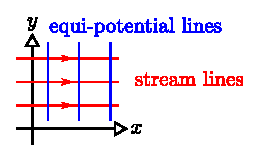
\includegraphics[scale=1.8]{figure/chapter5/5-1-1.eps}
%\caption{\label{fig:blue_rectangle} Rectangle}
\end{figure}
or
\begin{equation}
F(z) = Ve^{-i\alpha} z
\label{eq: 5-2-4}
\end{equation}
\begin{align*}
W(z) = \frac{dF}{dz}
&= Ve^{-i\alpha} \\
&= V\cos\alpha\mathbf{e_x} - iV\sin\alpha \mathbf{e_y}
\end{align*}
\begin{figure}[H]
\centering
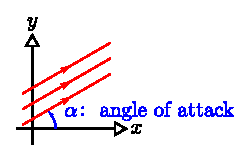
\includegraphics[scale=1.8]{figure/chapter5/5-1-2.eps}
%\caption{\label{fig:blue_rectangle} Rectangle}
\end{figure}
\item  Flow around a corner of arbitrary angle
\begin{equation}
F(z) = Az^n = A\left(re^{i\theta}\right)^n = Ar^ne^{in\theta}
\label{eq: 5-2-5}
\end{equation}
where $n$ is positive and $A$ is real number $>0$\\
i.e. 
\[
\left\{
\begin{aligned}
\Phi &= Ar^n\cos n\theta \\
\Psi &= Ar^n\sin n\theta
\end{aligned}
\right.
\]
and
\begin{subequations}
\begin{align}[left = \empheqlbrace\,]
v_r = \frac{\partial\Phi}{\partial r} &= nAr^{n-1}\cos n\theta \label{eq: 5-2-6a} \\
v_\theta = \frac{1}{r}\frac{\partial\Phi}{\partial \theta} &= -nAr^{n-1}\sin n\theta  \label{eq: 5-2-6b}
\end{align}
\end{subequations}
\begin{figure}[H]
\centering
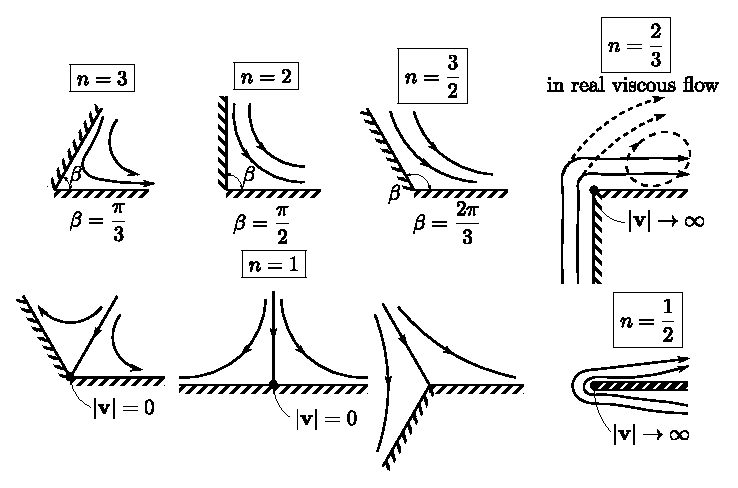
\includegraphics[scale=1.4]{figure/chapter5/5-1-3.eps}
%\caption{\label{fig:blue_rectangle} Rectangle}
\end{figure}
\[
\boxed{\beta = \frac{\pi}{n}}
\]
\item Plane (Line) Source/Sink
\begin{figure}[H]
\centering
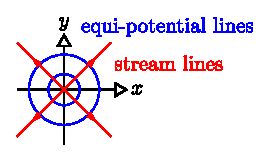
\includegraphics[scale=1.8]{figure/chapter5/5-1-4.eps}
%\caption{\label{fig:blue_rectangle} Rectangle}
\end{figure}
\begin{align}
F(z) &= m\ln z \label{eq: 5-2-7} \\
&=m\ln\left(re^{i\theta}\right) = m\ln r + im\theta\nonumber
\end{align}
where $m$ is real number, $m\colon +\longrightarrow$ source, $m\colon -\longrightarrow$ sink
\begin{subequations}
\begin{align}[left = \empheqlbrace\,]
\Phi &= m\ln r \label{eq: 5-2-8a}\\
\Psi &= m\theta \label{eq: 5-2-8b}
\end{align}
\end{subequations}
\begin{subequations}
\begin{align}[left = \empheqlbrace\,]
v_r &= \frac{m}{r} \label{eq: 5-2-9a}\\
v_\theta &= 0 \label{eq: 5-2-9b}
\end{align}
\end{subequations}
volume flow rate is
\[
Q = \oint_C\mathbf{v}\cdot\mathbf{n}dl = \int_0^{2\pi}v_rrd\theta = \int_0^{2\pi}\frac{m}{r}rd\theta = 2\pi m
\]
or 
\begin{equation}
F(z) = \frac{Q}{2\pi}\ln z
\label{eq: 5-2-10}
\end{equation}
If the origin of the source/sink is at $z_0$
\begin{equation}
F(z) = m\ln\left(z-z_0\right) = \frac{Q}{2\pi}\ln \left(z-z_0\right)
\label{eq: 5-2-11}
\end{equation}
\item Plane (Line) Vortex
\begin{figure}[H]
\centering
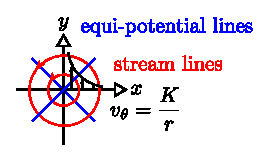
\includegraphics[scale=1.8]{figure/chapter5/5-1-5.eps}
%\caption{\label{fig:blue_rectangle} Rectangle}
\end{figure}
\begin{align}
F(z) &= -iK\ln z \label{eq: 5-2-12} \\
&=K\theta - iK\ln r\nonumber
\end{align}
where $K$ is real number.
\begin{subequations}
\begin{align}[left = \empheqlbrace\,]
\Phi &= K\theta \label{eq: 5-2-13a}\\
\Psi &= -K\ln r \label{eq: 5-2-13b}
\end{align}
\end{subequations}
\begin{subequations}
\begin{align}[left = \empheqlbrace\,]
v_r &= 0 \label{eq: 5-2-14a}\\
v_\theta &= \frac{K}{r} \label{eq: 5-2-14b}
\end{align}
\end{subequations}
Circulation is
\[
\Gamma = \oint_C\mathbf{v}\cdot\mathbf{t}dl = \int_0^{2\pi}v_\theta rd\theta = 2\pi K \neq 0
\]
or 
\begin{equation}
F(z) = -i\frac{\Gamma}{2\pi}\ln z
\label{eq: 5-2-15}
\end{equation}
If the origin of the vortex is at $z_0$
\begin{equation}
F(z) = -iK\ln\left(z-z_0\right) = -i\frac{\Gamma}{2\pi}\ln \left(z-z_0\right)
\label{eq: 5-2-16}
\end{equation}
\vspace{15em}
\item Plane (Line) Doublet (Dipole)
\vspace{5em}
\begin{figure}[H]
\centering
\begin{tikzpicture}[scale=2,transform canvas]
\draw [arrows = {-Latex[color=black, fill=white, length=3mm]}] (-2,0) -- (2,0) node [at end, above left] {$x$};
\draw [arrows = {-Latex[color=black, fill=white, length=3mm]}] (0,-2) -- (0,2) node [at end, left] {$y$};
\coordinate (P1) at (1,0);
\fill[color=black] (P1) circle[radius=2pt] node [below]{$m$(source)};
\coordinate (P2) at (-1,0);
\fill[color=black] (P2) circle[radius=2pt] node [below]{$-m$(sink)};
\draw[<->] (0,0.2) -- ($(P1)+(0,0.2)$) node [pos = 0.5, anchor=south]{$\epsilon$};
\draw[<->] (0,0.2) -- ($(P2)+(0,0.2)$) node [pos = 0.5, anchor=south]{$\epsilon$};
\end{tikzpicture}
\end{figure}
\vspace{5em}

\begin{align*}
F(z)
&= m\ln \left(z+\epsilon\right) - m\ln\left(z-\epsilon\right) \\
&= m\ln \frac{1+\epsilon/z}{1-\epsilon/z} \\
&= m\ln\left[1+2\frac{\epsilon}{z} + \mathcal{O}\left(\frac{\epsilon}{z}\right)^2\right] \\
&\cong m\left(2\frac{\epsilon}{z}\right)
\end{align*}
Let $\displaystyle\lim_{\epsilon\to 0}\left(2\epsilon m\right) = \mu$ where $\mu$ is real number
\begin{align}
\therefore 
F(z) &= \frac{\mu}{z} \label{eq: 5-2-17} \\
&= \frac{\mu}{re^{i\theta}} = \frac{\mu}{r}\cos\theta - i\frac{\mu}{r}\sin\theta \nonumber
\end{align}
\begin{subequations}
\begin{align}[left = \empheqlbrace\,]
\Phi &= \frac{\mu}{r}\cos\theta \label{eq: 5-2-18a}\\
\Psi &= -\frac{\mu}{r}\sin\theta \label{eq: 5-2-18b}
\end{align}
\end{subequations}
\begin{subequations}
\begin{align}[left = \empheqlbrace\,]
v_r &= -\frac{\mu}{r^2}\cos\theta \label{eq: 5-2-19a}\\
v_\theta &= -\frac{\mu}{r^2}\sin\theta \label{eq: 5-2-19b}
\end{align}
\end{subequations}
If origin of doublet is at $z-z_0$, then
\begin{equation}
F(z) = \frac{\mu}{z-z_0}
\label{eq: 5-2-20}
\end{equation}
\begin{figure}[H]
\centering
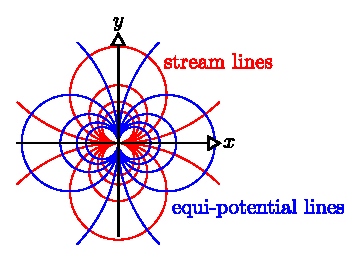
\includegraphics[scale=1.8]{figure/chapter5/5-1-6.eps}
%\caption{\label{fig:blue_rectangle} Rectangle}
\end{figure}
\begin{note}\mbox{}\\
\begin{enumerate}[label = \protect\circled{\arabic*}]
\item $\displaystyle\frac{d}{dz}\underbrace{\left(m\ln z\right)}_{=\text{source/sink}} = \underbrace{\frac{m}{z}}_{=\text{doublet}}$
\item $\displaystyle\frac{d}{dz}\underbrace{\left(\frac{m}{z}\right)}_{=\text{doublet}} = \underbrace{-\frac{m}{z^2}}_{=\text{quadruplet}}$
\begin{figure}[H]
\centering
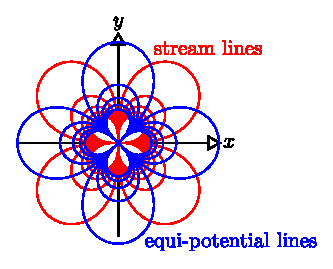
\includegraphics[scale=1.8]{figure/chapter5/5-1-7.eps}
%\caption{\label{fig:blue_rectangle} Rectangle}
\end{figure}
\item $\displaystyle\frac{1}{z^2},\frac{1}{z^3},\frac{1}{z^4},\cdots\colon$higher-order singularities
\end{enumerate}
\end{note}
\end{itemize}
\subsection{Images-Superposition}
\begin{itemize}
\item A singularities (source/sink, vortex, doublet, etc...) near an infinite plane wall
\begin{itemize}
\item source/sink
\begin{align*}
F(z) 
&= m\ln\left(z-ia\right) + m\ln\left(z+ia\right) \\
&= m\ln\left(z^2+a^2\right)
\end{align*}
\begin{figure}[H]
\centering
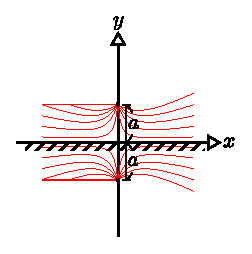
\includegraphics[scale=1.8]{figure/chapter5/5-1-8.eps}
%\caption{\label{fig:blue_rectangle} Rectangle}
\end{figure}
\item vortex
\begin{align*}
F(z) 
&= -\frac{i\Gamma}{2\pi}\ln\left(z-ia\right) + \frac{i\Gamma}{2\pi}\ln\left(z+ia\right) \\
&= \frac{i\Gamma}{2\pi}\ln\left(\frac{z+ia}{z-ia}\right)
\end{align*}
\begin{figure}[H]
\centering
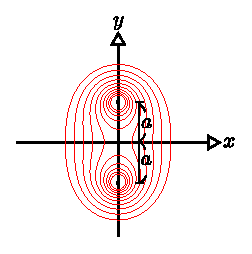
\includegraphics[scale=1.8]{figure/chapter5/5-1-9.eps}
%\caption{\label{fig:blue_rectangle} Rectangle}
\end{figure}
\end{itemize}
\item A singularity confined between two infinite plane walls\\
An infinite row of images of source 
\[
F(z) = m\sum_{n=-\infty}^{\infty}\ln\left(z+i2na\right)
\]
\begin{figure}[H]
\centering
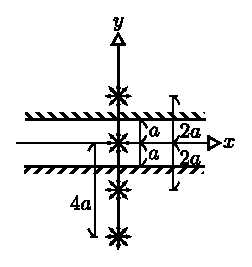
\includegraphics[scale=1.8]{figure/chapter5/5-1-10.eps}
%\caption{\label{fig:blue_rectangle} Rectangle}
\end{figure}
\item Distortion due to image
\begin{figure}[H]
\centering
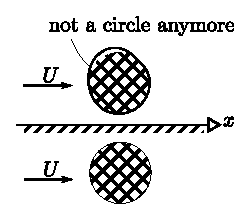
\includegraphics[scale=1.8]{figure/chapter5/5-1-11.eps}
%\caption{\label{fig:blue_rectangle} Rectangle}
\end{figure}
ref: A. B. Basset. On the motion of two spheres in a liquid, and allied problems. Proceedings of the London Mathematical Society
\end{itemize}
\subsection{Superposition-Flow around a circular cylinder with/without circulation}
\begin{itemize}
\item without circulation\\
Uniform stream + doublet: 
\[
F(z) = Uz + \frac{\mu}{z}
\]
require $r=a$ a streamline, then 
\[
F(ae^{i\theta}) = \left(Ua+ \frac{\mu}{a}\right)\cos\theta + i\left(Ua- \frac{\mu}{a}\right)\sin\theta
\]
\[
\Psi = \left(Ua - \frac{\mu}{a}\right)\sin\theta\Longrightarrow\Psi = 0\Longrightarrow\mu = Ua^2
\]
thus
\begin{equation}
F(z) = U\left(z + \frac{a^2}{z}\right)
\label{eq: 5-2-21}
\end{equation}
\begin{figure}[H]
\centering
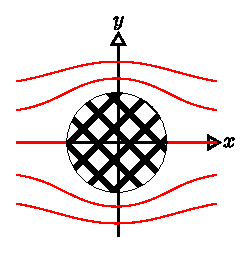
\includegraphics[scale=1.8]{figure/chapter5/5-1-12.eps}
%\caption{\label{fig:blue_rectangle} Rectangle}
\end{figure}
\item with circulation $\Gamma$\\
Can add a CW free vortex of strength $\Gamma$ to the above $F(z)$, i.e. uniform flow + doublet + vortex: 
\[
F(z) = U\left(z + \frac{a^2}{z}\right) + \frac{i\Gamma}{2\pi}\ln z + C
\]
require $r=a$ a streamline, then 
\begin{align*}
F(ae^{i\theta}) 
&= U\left(ae^{i\theta} + ae^{-i\theta}\right) + \frac{i\Gamma}{2\pi}\ln\left(ae^{i\theta}\right) + C \\
&= 2Ua\cos\theta - \frac{\Gamma\theta}{2\pi} + \frac{i\Gamma}{2\pi}\ln a + C
\end{align*}
choose $\displaystyle C = -\frac{i\Gamma}{2\pi}\ln a$, i.e. 
\begin{equation}
F(z) = U\left(z + \frac{a^2}{z}\right) + \frac{i\Gamma}{2\pi}\ln\frac{z}{a}
\label{eq: 5-2-22}
\end{equation}
\begin{subequations}
\begin{align}[left = \empheqlbrace\,]
\Phi &= U\cos\theta\left(r-\frac{a^2}{r}\right) - \frac{\Gamma\theta}{2\pi} \label{eq: 5-2-23a}\\
\Psi &= U\sin\theta\left(r-\frac{a^2}{r}\right) + \frac{\Gamma}{2\pi}\ln\frac{r}{a} \label{eq: 5-2-23b}
\end{align}
\end{subequations}
\begin{subequations}
\begin{align}[left = \empheqlbrace\,]
v_r &= U\cos\theta\left(1 - \frac{a^2}{r^2}\right) \label{eq: 5-2-24a}\\
v_\theta &= -U\sin\theta\left(1 + \frac{a^2}{r^2}\right) - \frac{\Gamma}{2\pi r} \label{eq: 5-2-24b}
\end{align}
\end{subequations}
On the surface of the circular cylinder  ($r=a$)
\[
\Longrightarrow
\left\{
\begin{aligned}
v_r &= 0 \\
v_\theta &= -2U\sin\theta - \frac{\Gamma}{2\pi a}
\end{aligned}
\right.
\]
Stagnation points
\begin{equation}
\Longrightarrow
\left\{
\begin{aligned}
v_r &= 0 \\
v_\theta &= 0
\end{aligned}
\right.
\Longrightarrow\sin\theta_s = -\frac{\Gamma}{4\pi Ua}
\label{eq: 5-2-25}
\end{equation}
\begin{figure}[H]
\centering
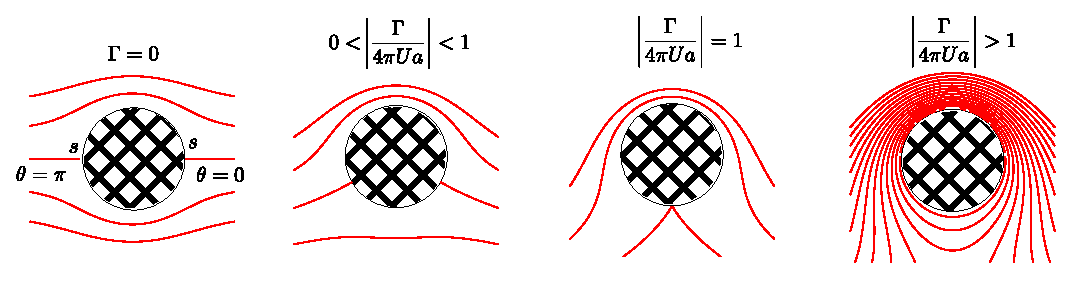
\includegraphics[scale=1.0]{figure/chapter5/5-1-13.eps}
%\caption{\label{fig:blue_rectangle} Rectangle}
\end{figure}
\end{itemize}
\subsection{The Circle Theorem (First)}
\begin{itemize}
\item Let $F(z)$ be the complex potential of a potential flow in the absence of any rigid boundaries and let all singularities of $F(z)$ be outside the circle $\abs{z} = a$.\\
If a circular cylinder $\abs{z} = a$ is introduced into the base flow $F(z)$, then the resulting complex potential $f(z)$ is given by 
\begin{equation}
f(z) = F(z) + \overline{F}(\frac{a^2}{z})\text{ (circle theorem)}
\label{eq: 5-2-26}
\end{equation}
\begin{proof}\mbox{}\\
\begin{enumerate}[label = \protect\circled{\arabic*}]
\item All singularities in $F(z)$ will lie inside the circle $\abs{z} = a$ in $\displaystyle\overline{F}(\frac{a^2}{z})$
\item If $z$ is on the circle $\abs{z} = a$, then $a^2/z = \bar{z}$, then 
\[
f(z) = F(z) + \overline{F}(\bar{z}) = \text{ real function}
\]
$\Longrightarrow\Psi = 0$ on $\abs{z} = a$, i.e. $\abs{z} =a$ is a streamline.
\end{enumerate}
\end{proof}
\begin{example}\mbox{}\\
\begin{figure}[H]
\centering
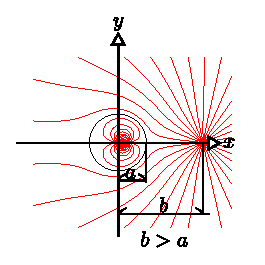
\includegraphics[scale=1.8]{figure/chapter5/5-1-14.eps}
%\caption{\label{fig:blue_rectangle} Rectangle}
\end{figure}
\[
F(z) = m\ln (z-b)
\]
\[
\Longrightarrow f(z) = m\ln\left(z-b\right) + m\ln\left(\frac{a^2}{z} - b\right)
\]
\end{example}
\end{itemize}
\subsection{Uniform Flow Past a Cylinder of Arbitrary Cross-Section}
\begin{itemize}
\item In general
\begin{align}
u - iv \equiv W(z) 
&\equiv\frac{dF(z)}{dz} = A_0 + \frac{A_1}{z} + \frac{A_2}{z^2} + \cdots\text{ (Laurent Series)}\nonumber \\
&= \sum_{n=0}^{\infty}\frac{A_n}{z_n}
\label{eq: 5-2-31}
\end{align}
\begin{equation}
\Longrightarrow
F(z) = \underbrace{A_0z}_{
\begin{subarray}{c}
  \text{uniform}\\
  \text{stream}
\end{subarray}
} + \underbrace{A_1\ln z}_{
\begin{subarray}{c}
  \text{source/sink}\\
  \text{or} \\
  \text{vortex}
\end{subarray}
} - \sum_{n=2}^\infty\frac{A_n}{n-1}\frac{1}{z^{n+1}} + \cancelto{0}{C}
\label{eq: 5-2-32}
\end{equation}
An $n\geq 2$ determined by geometry
\item About $A_0$ and $A_1$ in \eqref{eq: 5-2-32}\\
\begin{figure}[H]
\centering
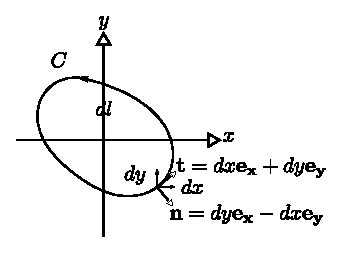
\includegraphics[scale=1.8]{figure/chapter5/5-1-15.eps}
%\caption{\label{fig:blue_rectangle} Rectangle}
\end{figure}
Note that 
\[
\Gamma = \ointctrclockwise_C\mathbf{v}\cdot\mathbf{t}dl = \ointctrclockwise_C\left(udx+vdy\right) = \ointctrclockwise_C d\Phi
\]
\[
Q = \ointctrclockwise_C\mathbf{v}\cdot\mathbf{n}dl = \ointctrclockwise_C\left(udy-vdx\right) = \ointctrclockwise_C d\Psi
\]
Hence 
\begin{align}
\Gamma + iQ
&= \ointctrclockwise_C\left(d\Phi + id\Psi\right)\nonumber \\
&= \ointctrclockwise_CdF = \ointctrclockwise_CW(z)dz\label{eq: 5-2-33}
\end{align}
In our present case, uniform free stream $U$ at $z\to\infty$. Hence $A_0 = U$ and
\begin{align*}
\Gamma + iQ
&= \ointctrclockwise_C W(z)dz \\
&= 0\text{ if $C$ does not enclose the cylinder}\\
&=2\pi iA_1\text{ for all circuits enclosing the cylinder}
\end{align*}
Let $A_1 = a_1 + ib_1$
\[
\Longrightarrow
\left\{
\begin{aligned}
\Gamma &= -2\pi b_1\Longrightarrow b_1 = -\frac{\Gamma}{2b} \\
Q &= 0 = 2\pi ia_1\Longrightarrow a_1 = 0
\end{aligned}
\right.
\]
for cylinder
\begin{equation}
W(z) = U - \frac{i\Gamma}{2\pi z} + \sum_{n=2}^\infty\frac{A_n}{z_n}
\label{eq: 5-2-34}
\end{equation}
\begin{equation}
F(z) = Uz - \frac{i\Gamma}{2\pi}\ln z + \sum_{n=2}^\infty\frac{A_n}{n-1}\frac{1}{z^{n-1}} + \cancelto{0}{C}
\label{eq: 5-2-35}
\end{equation}
\end{itemize}
\subsection{Force and Moment on a Cylinder}
\begin{itemize}
\item Blasius Theorem
\begin{figure}[H]
\centering
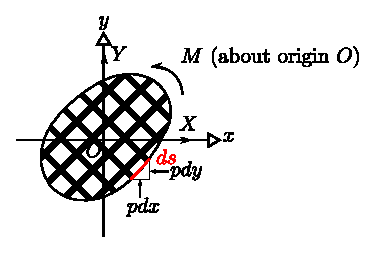
\includegraphics[scale=1.8]{figure/chapter5/5-1-16.eps}
%\caption{\label{fig:blue_rectangle} Rectangle}
\end{figure}
\begin{align*}
dX = -pdy, && dY = pdx, && dM = p\left(xdx + ydy\right)
\end{align*}
pressure: $p = p_\infty - \frac{\rho}{2}\abs{\mathbf{v}}^2$ can set $p_\infty = 0 $ without loss of generality.\\
Thus
\begin{align*}
d\left(X-iY\right) = \frac{\rho}{2}\abs{\mathbf{v}}^2\left(dy+idx\right), && dM = -\frac{\rho}{2}\abs{\mathbf{v}}^2\left(xdx + ydy\right)
\end{align*}
Now 
\begin{align*}
dy + idx = id\bar{z}, && xdx + ydy = \Re\left\{zd\bar{z}\right\}
\end{align*}
and 
\[
\abs{\mathbf{v}}^2 = W\overline{W} = \frac{dF}{dz}\frac{d\overline{F}}{d\bar{z}}
\]
Thus
\begin{align*}
d\left(X-iY\right) = \frac{\rho}{2}i\frac{dF}{dz}d\overline{F}, && dM = \Re\left\{-\frac{\rho}{2}z\frac{dF}{dz}d\overline{F}\right\}\text{ along $C$}
\end{align*}
On the cylinder, $\Psi = $ constant, $d\Psi = 0$\\
therefore
\[
d\overline{F} = d\left(\Phi - i\Psi\right) = d\left(\Phi + i\Psi\right) = dF = \frac{dF}{dz}dz
\]
along the cylinder surface\\
hence
\begin{align*}
d\left(X-iY\right) = \frac{\rho}{2}i\left(\frac{dF}{dz}\right)^2dz, && dM = \Re\left\{-\frac{\rho}{2}z\left(\frac{dF}{dz}\right)^2dz\right\}\text{ along $C$}
\end{align*}
i.e.
\begin{subequations}
\begin{align}[left = \empheqlbrace\,]
X - iY &= \frac{i\rho }{2}\oint_C\left(\frac{dF}{dz}\right)^2dz \label{eq: 5-2-40a} \\
M &= \Re\left\{-\frac{\rho}{2}\oint_Cz\left(\frac{dF}{dz}\right)^2dz\right\}  \label{eq: 5-2-40b}
\end{align}
\end{subequations}
$C$ could be any closed curve enclosing the cylinder
\end{itemize}
\subsection{Kutta-Joukowski Theorem}
\begin{figure}[H]
\centering
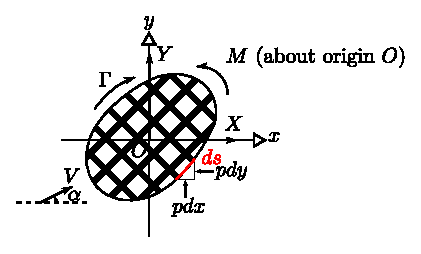
\includegraphics[scale=1.8]{figure/chapter5/5-1-17.eps}
%\caption{\label{fig:blue_rectangle} Rectangle}
\end{figure}
\begin{itemize}
\item Consider a cylinder (of arbitrary cross-section) placed in a uniform stream of speed $V$ at an angle-of-attack $\alpha$ with CW circulation of strength $\Gamma$. 
\begin{equation}
F(z) = Ve^{-i\alpha}z + \frac{i\Gamma}{2\pi}\ln z - \sum_{n=2}^{\infty}\frac{A_n}{n-1}\frac{1}{z^{n-1}}
\label{eq: 5-2-42}
\end{equation}
\[
\Longrightarrow W(z) = \frac{dF}{dz} = Ve^{-i\alpha} + \frac{i\Gamma}{2\pi z} + \sum_{n=2}^{\infty}\frac{A_n}{z^n}
\]
\[
\therefore W^2 = \underbrace{V^2e^{-2i\alpha}}_{B_0} + \underbrace{\frac{i\Gamma Ve^{-i\alpha}}{\pi}}_{B_{-1}}\frac{1}{z} + \underbrace{\frac{-\Gamma^2 + 8\pi^2A_2Ve^{-i\alpha}}{4\pi^2}}_{B_{-2}}\frac{1}{z^2} + \cdots
\]
From Blasius Theorem
\begin{align}
X - iY
&= \frac{i\rho}{2}\oint_CW^2(z)dz = \frac{i\rho}{2}2\pi i \left[B_{-1}\right]\nonumber \\
&= \frac{i\rho}{2}2\pi i\left(\frac{i\Gamma Ve^{-i\alpha}}{\pi}\right)\nonumber \\
&= -i\rho V e^{-i\alpha}\Gamma
\label{eq: 5-2-44}
\end{align}
or 
\begin{equation}
X + iY = \overline{X-iY} = i\rho V e^{-i\alpha}\Gamma
\label{eq: 5-2-45}
\end{equation}
In Aerodynamic:
\begin{align*}
\text{Lift force } L &\text{ is }\perp\text{ to free stream} \\
\text{Drag force } L &\text{ is }\parallel\text{ to free stream}
\end{align*}
\begin{equation}
D + iL = \left(X+iY\right)e^{-i\alpha} = i\rho V\Gamma
\label{eq: 5-2-46}
\end{equation}
\begin{subequations}
\begin{align}[left = \empheqlbrace\,]
L &= \rho V \Gamma\text{ (Kutta-Joukowski Theorem)} \label{eq: 5-2-47a} \\
D &= 0\text{ (d'Alembert paradox)}  \label{eq: 5-2-47b}
\end{align}
\end{subequations}
\item Moment on the cylinder 
\begin{align*}
M &= \Re\left\{-\frac{\rho}{2}\oint_CzW^2(z)dz\right\} = -\frac{\rho}{2}\Re\left\{2\pi i B_{-2}\right\} = \cdots \\ 
&= -2\pi \rho V\Re\left\{iA_2e^{-i\alpha}\right\}
\end{align*}

\end{itemize}
\section{Potential Flows Generated by Transformations}
\subsection{Conformal Transform (Mapping)}
General Properties
\begin{itemize}
\item Transformation (mapping) by analytic functions
\begin{figure}[H]
\centering
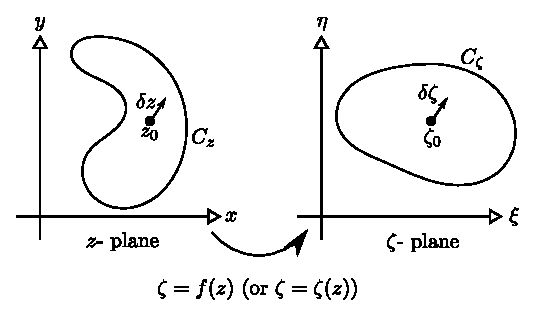
\includegraphics[scale=1.8]{figure/chapter5/5-1-18.eps}
%\caption{\label{fig:blue_rectangle} Rectangle}
\end{figure}
\begin{figure}[H]
\centering
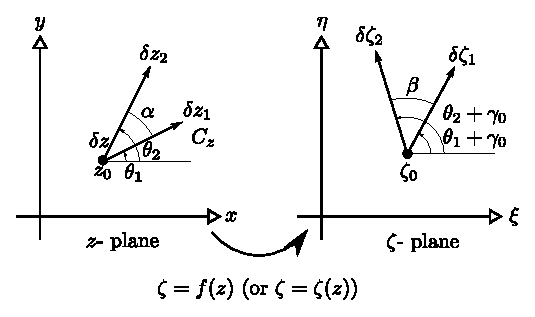
\includegraphics[scale=1.8]{figure/chapter5/5-1-19.eps}
%\caption{\label{fig:blue_rectangle} Rectangle}
\end{figure}
Assume $f(z)$ is analytic function and $\displaystyle\frac{d\zeta}{dz} = 0$, then 
\[
\delta\zeta = \left(\frac{d\zeta}{dz}\right)_{z_0}\delta z
\Longrightarrow\abs{\delta\zeta} = a_0\abs{\delta z},\arg(\delta\zeta) = \gamma_0+\arg(\delta z)\]
\[
\beta = \left(\theta_2+\gamma_0\right) - \left(\theta_1+\gamma_0\right) = \theta_2-\theta_1 = \alpha
\]
angle is preserved under mapping $\Longrightarrow$ Conformal mapping\\
What if $\boxed{\frac{d\zeta}{dz}=0} $ (critical point)
\item Analysis of the critical point of a transformation\\
Consider the transformation of form: 
\begin{align*}
\zeta = \left(z-z_0\right)^n \text{ ($n>1,n\colon$ integer)}, && \frac{d\zeta}{dz} = n\left(z-z_0\right)^{n-1}
\end{align*}
hence equal to zero at $z=z_0$
\begin{figure}[H]
\centering
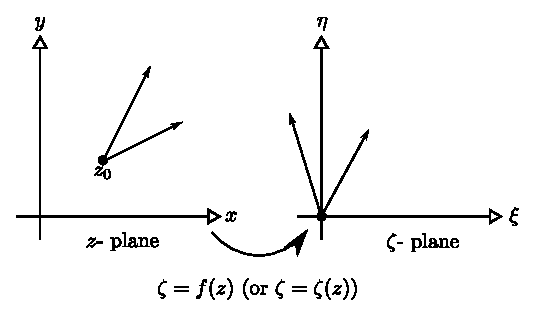
\includegraphics[scale=1.8]{figure/chapter5/5-1-20.eps}
%\caption{\label{fig:blue_rectangle} Rectangle}
\end{figure}
Let $z-z_0 = re^{i\theta}$, $\zeta = \rho e^{i\phi}$, then 
\begin{align*}
\zeta = \left(z-z_0\right)^n
&\Longrightarrow \rho e^{i\phi} = r^ne^{in\theta} \\
&\Longrightarrow \rho = r^n, \phi = n\theta\Longrightarrow\beta = n\alpha
\end{align*}
angle is not preserved at critical point under mapping.\\
Now consider the general transformation $\zeta = \zeta (z)$ and $z_0$ is a critical point
\[
\zeta(z) = \zeta(z_0) + a_1\left(z-z_0\right) + a_2\left(z-z_0\right)^2 + \cdots
\]
where
\[
a_k = \frac{1}{k!}\left(\frac{d^k\zeta}{dz^k}\right)_{z=z_0}
\]
Let us suppose the first $\left(n-1\right)$ derivatives are zero, i.e.
\[
a_1 = a_2 = a_3 = \cdots = a_{n-1} = 0,a_n\neq 0
\]
then
\[
\zeta = \zeta_0 + a_n\left(z - z_0\right)^n\overbrace{\left[1 + \frac{a_{n+1}}{a_n}\left(z-z_0\right) + \frac{a_{n+2}}{a_n}\left(z-z_0\right)^2 + \cdots\right]}^{f(z-z_0)}
\]
$\Longrightarrow \zeta-\zeta_0 = \left(z-z_0\right)^nf(z-z_0)$ as $z\to z_0$, $f(z-z_0)\approx 1 + O(z-z_0)$
\begin{example}\mbox{}\\
\begin{figure}[H]
\centering
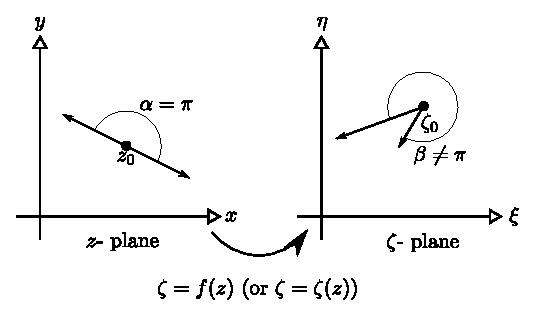
\includegraphics[scale=1.8]{figure/chapter5/5-1-21.eps}
%\caption{\label{fig:blue_rectangle} Rectangle}
\end{figure}
smooth curve will map to a sharp corner at critical point.
\end{example}
\item Application to the Potential Flow
\begin{enumerate}[label = (\alph*)]
\item \label{ch5-3-1-a} Consider a potential flow over certain configuration $C_z$ an $z$- plane with a complex potential $F(z)=\Phi(x,y) + i\Psi(x,y)$, suppose a conformal transformation $\zeta = \zeta(z)$, $\zeta = \xi + i\eta$, $z = x+iy$, which maps $C_z$ on $z$- plane into a relatively simple configuration $C_\zeta$ (e.g. a circle) on $\zeta$- plane.
\begin{figure}[H]
\centering
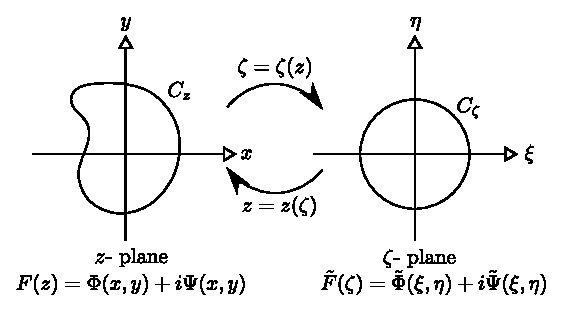
\includegraphics[scale=1.8]{figure/chapter5/5-1-22.eps}
%\caption{\label{fig:blue_rectangle} Rectangle}
\end{figure}
\begin{equation}
\tilde{F}(\zeta) = F(z(\zeta))
\label{eq: 5-3-1}
\end{equation}
Now
\[
\frac{d\tilde{F}}{d\zeta} = \frac{dF}{dz}\frac{dz}{d\zeta} = \frac{dF}{dz}/\frac{d\zeta}{dz}
\]
exists at all points where $d\zeta/dz\neq 0$\\
$\Longrightarrow\tilde{F}(\zeta)$ is an analytic function except at critical point of transformation.
\item The complex velocity on $\zeta$- plane
\begin{equation}
\tilde{W}(\zeta) = \frac{d\tilde{F}}{d\zeta} = \frac{dF}{dz}/\frac{d\zeta}{dz} = W(z)/\frac{d\zeta}{dz}
\label{eq: 5-3-2}
\end{equation}
$\tilde{W}(\zeta)\to\infty$ at the critical point $\displaystyle\frac{d\zeta}{dz} = 0$
\item Transformation of uniform condition at $\infty$
\begin{align*}
\frac{dz}{d\zeta}\to 1 &&\text{as}&&\zeta\to\infty
\end{align*}
i.e.
\begin{align*}
z\longleftrightarrow\zeta &&\text{as}&&\zeta\to\infty
\end{align*}
hence the form of the transformation
\[
z(\zeta) = \zeta + \frac{c_1}{\zeta} + \frac{c_2}{\zeta^2} + \cdots + = \zeta + \sum_{n=1}^\infty\frac{c_n}{\zeta^n}
\]
\item \label{ch5-3-1-d}
\begin{align*}
\Gamma_\zeta + iQ_\zeta
&= \oint_{C_\zeta}\overline{W}(\zeta)d\zeta = \oint_{C_\zeta}\frac{d\overline{F}}{d\zeta}d\zeta \\
&= \oint_{C_z}\frac{dF}{dz}\frac{dz}{d\zeta}d\zeta \\
&= \oint_{C_z}W(z)dz = \Gamma_z + iQ_z
\end{align*}
\end{enumerate}
Based on \ref{ch5-3-1-a}$\sim$\ref{ch5-3-1-d}
\begin{example}\mbox{}\\
Transformation of a uniform stream past a circular cylinder on $\zeta$- plane into that past an arbitrary cylinder on $z$- plane
\begin{equation}
z = \zeta + \frac{c_1}{\zeta} + \frac{c_2}{\zeta^2} + \cdots
\label{eq: 5-3-4}
\end{equation}
an from Blasius Theorem
\begin{equation}
\begin{aligned}
X - iY
&= \frac{i\rho}{2}\oint_{C_z}W^2(z)dz \\
&= \frac{i\rho}{2}\oint_{C_\zeta}W^2(\zeta)\left(\frac{d\zeta}{dz}\right)^2dz \\
&= \frac{i\rho}{2}\oint_{C_\zeta}W^2(\zeta)\frac{1}{dz/d\zeta}d\zeta
\end{aligned}
\label{eq: 5-3-5}
\end{equation}
\begin{equation}
\begin{aligned}
M
&= -\frac{\rho}{2}\Re\left\{\oint_{C_z}zW^2(z)dz\right\} \\
&= -\frac{\rho}{2}\Re\left\{\oint_{C_\zeta}z(\zeta)W^2(\zeta)\frac{1}{dz/d\zeta}d\zeta\right\}
\end{aligned}
\label{eq: 5-3-6}
\end{equation}
\end{example}
\end{itemize}
\subsection{Joukowski Transformation}
\begin{itemize}
\item General properties of J-T
\begin{equation}
z = \zeta + \frac{c^2}{\zeta}\text{ (J-T)}
\label{eq: 5-3-7}
\end{equation}
\begin{equation}
\frac{dz}{d\zeta} = 1 - \frac{c^2}{\zeta^2}
\label{eq: 5-3-8}
\end{equation}
As $\zeta\to \infty$, $\displaystyle\frac{dz}{d\zeta}\to 1$, i.e. $z\to\zeta$\\
A singular point at $\zeta = 0$; Two critical points at $\zeta = \pm c$
\begin{figure}[H]
\centering
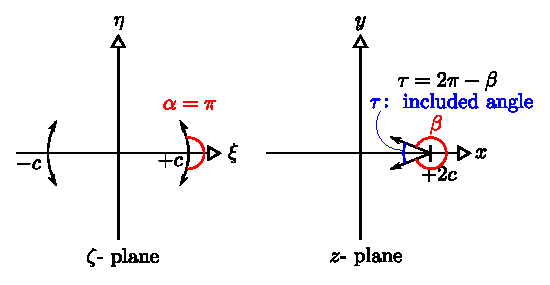
\includegraphics[scale=1.8]{figure/chapter5/5-1-23.eps}
%\caption{\label{fig:blue_rectangle} Rectangle}
\end{figure}
Previously, we have $\boxed{\beta = n\alpha}$\\
i.e. $2\pi-\tau = n\alpha\Longrightarrow \beta = n\alpha\Longrightarrow\tau = 2\pi -n\alpha$ where $n$ is the order of derivatives, i.e, $\displaystyle\frac{d^nz}{d\zeta^n}$ that first becomes non-zero.\\
\vspace{1em}
%----------------------
\begin{minipage}{0.4\textwidth}
For J-T, $n\equiv 2$, $\therefore\tau = 2\pi -n\alpha = 0$
\end{minipage} \hfill
\begin{minipage}{0.4\textwidth}
\begin{tikzpicture}[scale=2,transform canvas]
    \draw [color=black, -, rotate=0] ($(0,0.2)$) arc [start angle=210, end angle=270, x radius=1.2cm, y radius=0.6cm] node[above]{$\tau = 0$};
    \draw [color=black, -, rotate=0] ($(0,-0.4)$) arc [start angle=150, end angle=90, x radius=1.2cm, y radius=0.6cm] node[below]{\underline{cusp}};
\end{tikzpicture}
\end{minipage}\\
%----------------------
\end{itemize}
\subsection{Families of J-T}
\begin{enumerate}[label = (\alph*)]
\item Flow around elliptic cylinder \label{ch5-3-a}\\
Consider a circle of radius $a$ ($a>c$), centred at origin on $\zeta$- plane
\begin{figure}[H]
\centering
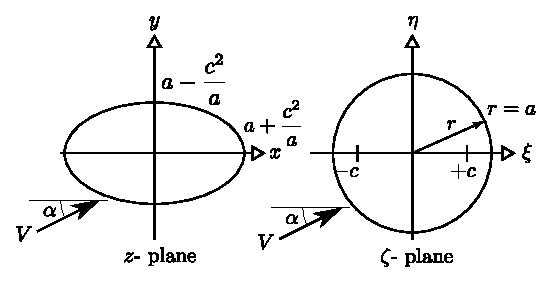
\includegraphics[scale=1.8]{figure/chapter5/5-1-24.eps}
%\caption{\label{fig:blue_rectangle} Rectangle}
\end{figure}
J-T
\begin{align*}
z = \zeta + \frac{c^2}{\zeta}, && \zeta = ae^{i\theta}
\end{align*}
\begin{align*}
\Longrightarrow
z 
&= ae^{i\theta} + \frac{c^2}{ae^{i\theta}} \\
&= \left(a + \frac{c^2}{a}\right)\cos\theta + i\left(a - \frac{c^2}{a}\right)\sin\theta \\
&= x + iy
\end{align*}
\[
\Longrightarrow
\left\{
\begin{aligned}
x &= \left(a + \frac{c^2}{a}\right)\cos\theta \\
y &= \left(a - \frac{c^2}{a}\right)\sin\theta
\end{aligned}
\right.
\]
or
\[
\left(\frac{x}{a+c^2/a}\right)^2 - \left(\frac{y}{a-c^2/a}\right)^2 = 1
\]
It is an ellipse!\\
Consider a uniform stream of speed $V$ and angle-of-attack $\alpha$ past the circular cylinder on $\zeta$- plane
\begin{equation}
F(\zeta) = V\left(e^{-i\alpha}\zeta + \frac{a^2}{\zeta}e^{i\alpha}\right)
\label{eq: 5-3-11}
\end{equation}
From J-T
\[
\zeta^2 - z\zeta + c^2 = 0\Longrightarrow\zeta \vc{=}{\footnotemark}{} \frac{z}{2}\pm\sqrt{\left(\frac{z}{2}\right)^2-c^2}
\]
\begin{align*}
\therefore F(z)
&= F(\zeta(z)) \\
&= V\left\{\left[\frac{z}{2} + \sqrt{\left(\frac{z}{2}\right)^2-c^2}\right]e^{-i\alpha} + \frac{a^2e^{i\alpha}}{\frac{z}{2} + \sqrt{\left(\frac{z}{2}\right)^2-c^2}}\right\} \\
&=V\left[ze^{-i\alpha} + \left(\frac{a^2}{c^2}e^{i\alpha} - e^{-i\alpha}\right)\left(\frac{z}{2}-\sqrt{\left(\frac{z}{2}\right)^2 - c^2}\right)\right]
\end{align*}
\footnotetext{discard $-$ since $z\to\zeta$ as $\zeta\to\infty$}
\begin{figure}[H]
\centering
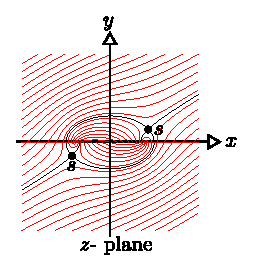
\includegraphics[scale=1.8]{figure/chapter5/5-1-25.eps}
%\caption{\label{fig:blue_rectangle} Rectangle}
\end{figure}
\begin{example}{Stagnation points on the ellipse}\mbox{}\\
$\zeta = \pm ae^{i\alpha}$ subs into J-T 
\begin{equation}
z = \zeta + \frac{c^2}{\zeta}\Longrightarrow z = \pm \left(a + \frac{c^2}{a}\right)\cos\alpha \pm i\left(a - \frac{c^2}{a}\right)\sin\alpha
\end{equation}
\end{example}
\item Flow around a flat plate \label{ch5-3-b}
\begin{figure}[H]
\centering
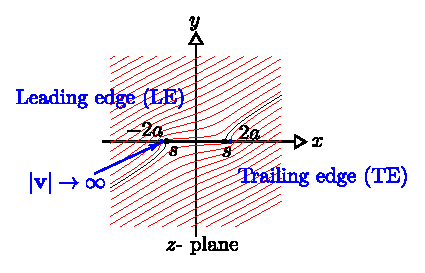
\includegraphics[scale=1.8]{figure/chapter5/5-1-26.eps}
%\caption{\label{fig:blue_rectangle} Rectangle}
\end{figure}
In \ref{ch5-3-a}, let $c=a$, the $\zeta = ae^{i\theta}\vc{\Longrightarrow}{\text{maps to}}{}-2a\leq x\leq 2a$ on $z$- plane
\begin{equation}
F(z) = V\left[ze^{-i\alpha} + \left(e^{i\alpha} - e^{-i\alpha}\right)\left(\frac{z}{2}-\sqrt{\left(\frac{z}{2}\right)^2-a^2}\right)\right]
\end{equation}
\begin{example}{Stagnation points on the plate}\mbox{}\\
$\zeta = \pm ae^{i\alpha}$ subs into J-T 
\begin{equation}
z = \zeta + \frac{c^2}{\zeta}\Longrightarrow z = \pm 2a\cos\alpha 
\end{equation}
\end{example}
\item Flow around a circular arc (camber line) \label{ch5-3-c}
\begin{figure}[H]
\centering
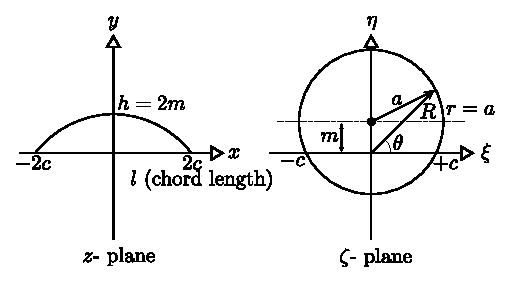
\includegraphics[scale=1.8]{figure/chapter5/5-1-27.eps}
%\caption{\label{fig:blue_rectangle} Rectangle}
\end{figure}
From $\zeta = R(\theta)e^{i\theta}$ and J-T: $\displaystyle z = Re^{i\theta} + \frac{c}{R^2}e^{-i\theta}$
\[
\Longrightarrow
\left\{
\begin{aligned}
x &= \left(R + \frac{c^2}{R}\right)\cos\theta \\
y &= \left(R - \frac{c^2}{R}\right)\sin\theta
\end{aligned}
\right.
\]
\begin{equation}
\vc{\Longrightarrow}{\text{eliminating}}{R}
x^2\sin^2\theta - y^2\cos^2\theta = 4c^2\sin^2\theta\cos^2\theta
\label{eq: 5-3-16}
\end{equation}
use relation
\begin{equation}
c^2+m^2 = a^2 = R^2 + m^2 - 2Rm\overbrace{\cos\left(\frac{\pi}{2}-\theta\right)}^{\sin\theta}
\tag{$\ast$}
\label{eq: 5-3-*}
\end{equation}
\begin{example}\mbox{}\\
\begin{equation}
\eqref{eq: 5-3-16}\Longrightarrow
x^2 + \left[y+c\left(\frac{c}{m}-\frac{m}{c}\right)\right]^2 = c^2\left[4+\left(\frac{c}{m}-\frac{m}{c}\right)^2\right]
\label{eq: 5-3-17}
\end{equation}
\begin{solution}\mbox{}\\
From \eqref{eq: 5-3-*}
\[
\sin\theta = \frac{R^2-c^2}{2Rm}\text{ and } \sin\theta= \frac{y}{R-c^2/R}\Longrightarrow\sin\theta = \frac{y}{2m\sin\theta}
\]
\begin{align*}
\Longrightarrow\sin^2\theta = \frac{y}{2m}, &&\cos^2\theta = 1-\sin^2\theta = 1-\frac{y}{2m}
\end{align*}
\end{solution}
\end{example}
\[
\eqref{eq: 5-3-17}\Longrightarrow
\left\{
\begin{aligned}
l &= 4c \\
h &= 2m
\end{aligned}
\right.
\Longrightarrow
\left\{
\begin{aligned}
c &= \frac{l}{4} \\
m &= \frac{h}{2}
\end{aligned}
\right.
\text{ If we let }\frac{m}{c} = \epsilon\ll 1
\]
then
\begin{subequations}
\begin{equation}
x^2 + \left(y+\frac{c^2}{m}\right)^2 = c^2\left(4+\frac{c^2}{m^2}\right) + \mathcal{O}(\epsilon^2)
\label{eq: 5-3-18a}
\end{equation}
correct to $\mathcal{O}(\epsilon)$\\
in terms of $l$ and $h$
\begin{equation}
x^2 + \left(y+\frac{l^2}{8h}\right)^2 = \frac{l^2}{4}\left(1+\frac{l^2}{16h^2}\right)
\label{eq: 5-3-18b}
\end{equation}
\end{subequations}
The complex potential is
\begin{equation}
F(\zeta) = V\left[\left(\zeta-im\right)e^{-i\alpha}+\frac{a^2}{\zeta-im}e^{i\alpha}\right]
\label{eq: 5-3-19}
\end{equation}
with
\[
z = \zeta + \frac{c^2}{\zeta}
\]
\begin{figure}[H]
\centering
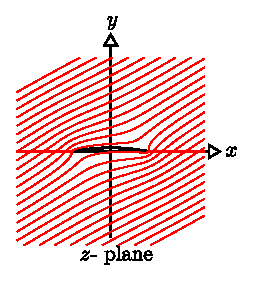
\includegraphics[scale=1.8]{figure/chapter5/5-1-28.eps}
%\caption{\label{fig:blue_rectangle} Rectangle}
\end{figure}
\item Flow around a symmetric Joukowski airfoil  \label{ch5-3-d}
\begin{figure}[H]
\centering
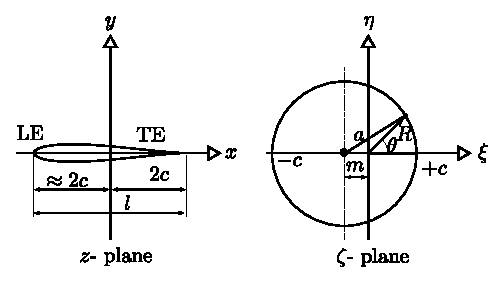
\includegraphics[scale=1.8]{figure/chapter5/5-1-29.eps}
%\caption{\label{fig:blue_rectangle} Rectangle}
\end{figure}
From J-T and infinitesimal assumption
\begin{align*}
z = \zeta + \frac{c^2}{\zeta}, && \epsilon = \frac{m}{c}\ll 1
\end{align*}
hence $\zeta = c\Longrightarrow z = 2c$
\[
\zeta = -\left(c+2m\right)\Longrightarrow z = -c\left(1+2\epsilon\right)-\frac{c}{1+2\epsilon} = -2c + \mathcal{O}(\epsilon^2)
\]
hence
\[
l\approx 4c + \mathcal{\epsilon^2}
\]
\begin{exercise}{Show that correct to $\mathcal{\epsilon}$, the airfoil shape on $z$- plane is given by}
\[
z\approx c\left[2\cos\theta+i2\epsilon\left(1-\cos\theta\right)\sin\theta\right] + \mathcal{O}(\epsilon^2)
\]
i.e.
\[
\left\{
\begin{aligned}
x &\approx 2c\cos\theta \\
y &\approx 2c\epsilon\left(1-\cos\theta\right)\sin\theta
\end{aligned}
\right.
\]
or
\begin{equation}
y \approx \pm 2c\epsilon\left(1-\frac{x}{2c}\right)\sqrt{1-\left(\frac{x}{2c}\right)^2} + \mathcal{O}(\epsilon^2)
\label{eq: 5-3-20}
\end{equation}
\begin{solution}\mbox{}\\
From cosine theorem
\begin{align*}
a^2 = \left(c+m\right)^2
&= R^2\left(1+\frac{m^2}{R^2} + 2\frac{m}{R}\cos\theta\right) \\
&\vc{=}{\footnotemark}{}R^2\left(1+2\underbrace{\frac{m}{R}}_{\mathcal{O}(\epsilon)}\cos\theta + \mathcal{O}(\epsilon^2)\right)
\end{align*}
\footnotetext{From $R\geq c$, $m/R\leq m/c$, i.e. $m/R=\mathcal{O}(\epsilon)$}
\[
\Longrightarrow c+m \approx R\left(1+\frac{m}{R}\cos\theta\right)
\]
\[
\therefore R\approx c\left[1+\epsilon\left(1-\cos\theta\right)\right]
\]
From J-T
\begin{align*}
z 
&= \zeta + \frac{c^2}{\zeta} \\
&= Re^{i\theta} + \frac{c^2}{R}e^{-i\theta} \\
&= c\left[1+\epsilon\left(1-\cos\theta\right)\right]e^{i\theta} + \frac{ce^{-i\theta}}{1+\epsilon\left(1-\cos\theta\right)} \\
&\vc{=}{\footnotemark}{}c\left[1+\epsilon\left(1-\cos\theta\right)\right]e^{i\theta} + c\left[1-\epsilon\left(1-\cos\theta\right)+\mathcal{O}(\epsilon^2)\right]e^{-i\theta}
\end{align*}
\footnotetext{$\displaystyle\frac{ce^{-i\theta}}{1+\epsilon\left(1-\cos\theta\right)} = ce^{-i\theta}\left[1-\epsilon\left(1-\cos\theta\right)+\mathcal{O}(\epsilon^2)\right]$}
\end{solution}
\end{exercise}
Maximum thickness $t$ occurs at $\displaystyle\frac{dy}{dx} = 0$
\[
\Longrightarrow
\left\{
\begin{aligned}
x & = -c \\
y & = \pm\frac{3\sqrt{3}}{2}c\epsilon
\end{aligned}
\right.
\Longrightarrow t\approx 3\sqrt{3}c\epsilon
\]
hence thickness ratio
\[
\frac{t}{l} = \frac{3\sqrt{3}}{4}\epsilon\Longrightarrow\epsilon = \frac{m}{c}\approx\frac{4}{3\sqrt{3}}\frac{t}{l} \approx 0.77\frac{t}{l}
\]
equation for the airfoil in terms of $t$ and $l$
\begin{equation}
\frac{y}{t}\approx\pm 0.385\left(1-2\frac{x}{l}\right)\sqrt{1-\left(\frac{2x}{l}\right)^2}
\label{eq: 5-3-21}
\end{equation}
The complex potential is
\begin{equation}
F(\zeta) = V\left[\left(\zeta+m\right)e^{-i\alpha} + \frac{a^2}{\zeta + m}e^{i\alpha}\right]
\label{eq: 5-3-22}
\end{equation}
\begin{figure}[H]
\centering
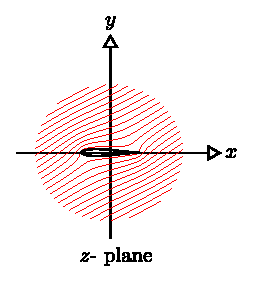
\includegraphics[scale=1.8]{figure/chapter5/5-1-30.eps}
%\caption{\label{fig:blue_rectangle} Rectangle}
\end{figure}
\item Flow around a cambered Joukowski airfoil\label{ch5-3-e}
\begin{figure}[H]
\centering
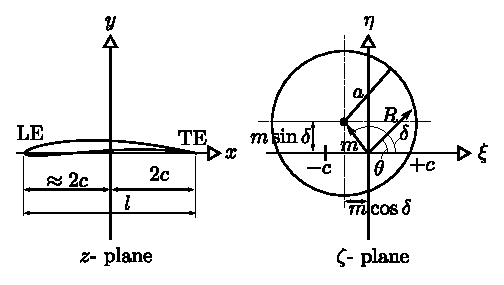
\includegraphics[scale=1.8]{figure/chapter5/5-1-31.eps}
%\caption{\label{fig:blue_rectangle} Rectangle}
\end{figure}
For $\epsilon = m/c\ll 1$\\
correct to $\mathcal{O}(\epsilon)$, equation of the cambered Joukowski airfoil
\begin{equation}
\begin{aligned}
y 
&= \underbrace{\sqrt{\frac{l^2}{4}\left(1+\frac{l^2}{16h^2}\right)-x^2}-\frac{l^2}{8h}}_{
\begin{subarray}{c}
  \text{equation for camber}\\
  \text{\eqref{eq: 5-3-18b}}
\end{subarray}
} \\
&\pm\underbrace{ 0.385\left(1-2\frac{x}{l}\right)\sqrt{1-\left(\frac{2x}{l}\right)^2} + \mathcal{O}(\frac{t}{l})^2}_{
\begin{subarray}{c}
  \text{equation for thickness}\\
  \text{\eqref{eq: 5-3-21}}
\end{subarray}
}
\end{aligned}
\label{eq: 5-3-23}
\end{equation}
The complex potential is
\begin{equation}
F(\zeta) = V\left[\left(\zeta - me^{i\delta}\right)e^{-i\alpha} + \frac{a^2e^{i\alpha}}{\zeta - me^{i\delta}}\right]
\label{eq: 5-3-24}
\end{equation}
with $\displaystyle z = \zeta + \frac{c^2}{\zeta}$ and
\begin{align*}
m\cos\delta\approx\frac{0.77}{4}t, && m\sin\delta\approx\frac{h}{2}, && a\approx\frac{l}{4}\left(1+0.77\frac{t}{l}\right)
\end{align*}
\end{enumerate}
\subsection{Kutta Condition}
Above \ref{ch5-3-b}$\sim$\ref{ch5-3-e} cases all involve a singular point at TE where velocity $\to\infty$. The viscous effect must take action.
\begin{itemize}
\item Kutta-Joukowski hypothesis\\
Whenever a flow passing around sharp corner, the viscous effect becomes significant and cannot be neglected therefore,\\
instead of 
\begin{figure}[H]
\centering
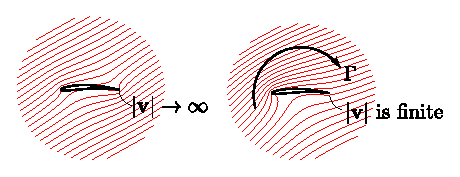
\includegraphics[scale=1.8]{figure/chapter5/5-1-32.eps}
%\caption{\label{fig:blue_rectangle} Rectangle}
\end{figure}
These should be a circulation around the airfoil as a manifestation of the viscous effect (flow separation), the magnitude of the circulation being such that to ensure the flow leave the TE smoothly, i.e.\\
$\Gamma$ is fixed by the requirement
\begin{equation}
\frac{dF(z)}{dz} = \frac{dF}{d\zeta}/\frac{dz}{d\zeta}\text{ is finite at TE}
\label{eq: 5-3-30}
\end{equation}
which implies
\begin{equation}
\frac{dF}{d\zeta} = 0\text{ at TE (at critical point $\zeta = c$)}
\label{eq: 5-3-31}
\end{equation}
\begin{figure}[H]
\centering
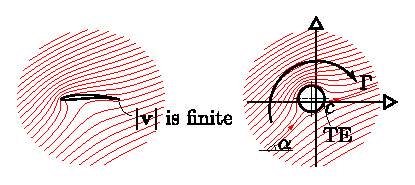
\includegraphics[scale=1.8]{figure/chapter5/5-1-33.eps}
%\caption{\label{fig:blue_rectangle} Rectangle}
\end{figure}
\item Generation of Stating Vortex and Bound Vortex \\
Consider
\begin{figure}[H]
\centering
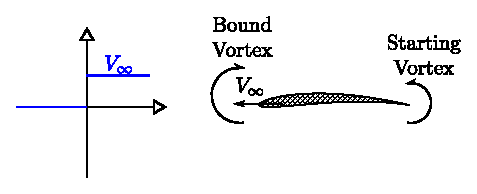
\includegraphics[scale=1.8]{figure/chapter5/5-1-34.eps}
%\caption{\label{fig:blue_rectangle} Rectangle}
\end{figure}
%----------------------
\begin{minipage}{0.1\textwidth}
\begin{figure}[H]
\centering
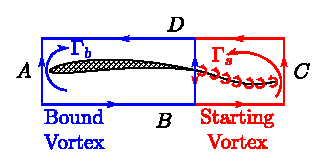
\includegraphics[scale=1.8]{figure/chapter5/5-1-35.eps}
%\caption{\label{fig:blue_rectangle} Rectangle}
\end{figure}
\end{minipage}\hfill
\begin{minipage}{0.35\textwidth}
From Kelvin's Theorem
\[
\frac{D\Gamma_{ABCD}}{Dt} = 0\Longrightarrow\Gamma_{ABCD} = 0
\]
\[
\Gamma_b-\Gamma_s = \Gamma_{ABCD} = 0
\]
\[
\Gamma_b = - \Gamma_s
\]
\end{minipage}\\
\vspace{2em}
%----------------------
\item Back to the Joukowski-airfoil problems
\begin{figure}[H]
\centering
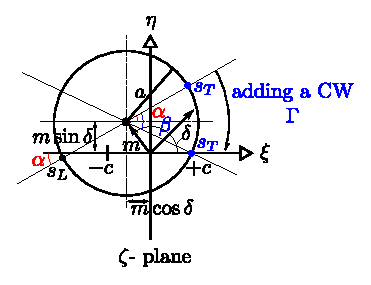
\includegraphics[scale=1.8]{figure/chapter5/5-1-36.eps}
%\caption{\label{fig:blue_rectangle} Rectangle}
\end{figure}
Recall 
\[
F(\zeta) = V\left[\left(\zeta-\zeta_0\right)e^{-i\alpha} + \frac{a^2e^{i\alpha}}{\zeta-\zeta_0}\right] + \frac{i\Gamma}{2\pi}\ln\left(\zeta-\zeta_0\right)
\]
\begin{equation}
W(\zeta) = \frac{dF}{d\zeta} = Ve^{-i\alpha} + \frac{i\Gamma}{2\pi}\frac{1}{\zeta - \zeta_0} - Ve^{i\alpha}a^2\frac{1}{\left(\zeta-\zeta_0\right)}
\label{eq: 5-3-32}
\end{equation}
From geometry: $c-\zeta_0 = ae^{-i\beta}$\\
at $TE$: $\zeta = c$
\[
W(c) = Ve^{-i\alpha} + \frac{i\Gamma}{2\pi}e^{i\beta} - Ve^{i\left(\alpha+2\beta\right)}
\]
KC require $W(c) = 0$
\[
\Longrightarrow 2\pi a V\left[1-e^{2i\left(\alpha+\beta\right)}\right] + i\Gamma e^{i\left(\alpha+\beta\right)} = 0
\]
\[
\Longrightarrow \Gamma = 4\pi a V\sin\left(\alpha+\beta\right)
\]
The lift on the Joukowski airfoil is
\begin{equation}
L = \rho V\Gamma = 4\pi a\rho V^2\sin\left(\alpha+\beta\right)
\label{eq: 5-3-33}
\end{equation}
the lift coefficient $C_L$ is defined as
\begin{equation}
C_L = \frac{L}{\frac{\rho}{2}V^2l} = 8\pi\left(\frac{a}{l}\right)\sin\left(\alpha+\beta\right)
\label{eq: 5-3-34}
\end{equation}
For small angle-of-attack, $\alpha\ll 1$, and small $\beta$ (which corresponds to \emph{thin} airfoil) $\beta\ll 1$,
\[
\sin\left(\alpha+\beta\right)\approx\alpha + \beta
\]
hence
\begin{equation}
L\approx 4\pi\rho V^2 a\left(\alpha+\beta\right)
\label{eq: 5-3-35}
\end{equation}
\begin{equation}
C_L\approx 8\pi\left(\frac{a}{l}\right)\left(\alpha+\beta\right)
\label{eq: 5-3-35}
\end{equation}
Furthermore, if $\beta \ll 1$, $l\approx 4c\approx 4a$, hence
\begin{equation}
L\approx \pi\rho lV^2\left(\alpha+\beta\right)
\label{eq: 5-3-36}
\end{equation}
\begin{equation}
\boxed{C_L\approx 2\pi\left(\alpha+\beta\right)}
\label{eq: 5-3-37}
\end{equation}
where $\alpha$ is angle-of-attack and $\beta$ is related to camber $\approx\displaystyle\frac{2h}{l}$
\begin{note}\mbox{}\\
\begin{enumerate}[label = \protect\circled{\arabic*}]
\item $L\neq 0$ at $\alpha = 0$ (due to camber) \\
\item $L = 0$ when $\alpha =-\beta$, $-\beta\equiv\alpha_0$, where $\alpha_0$ is zero-left angle \\
Define an effective angle-of-attack $\alpha_e$
\begin{align*}
\alpha_e = \alpha - \alpha_0 = \alpha + \beta, && C_L\approx 2\pi \alpha_e
\end{align*}
\end{enumerate}
\begin{figure}[H]
\centering
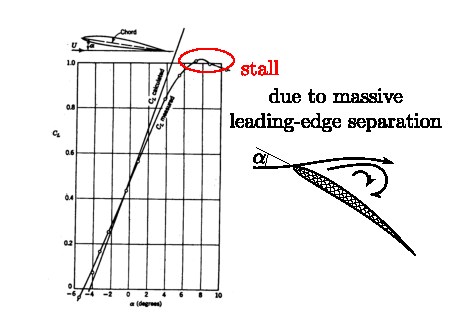
\includegraphics[scale=1.8]{figure/chapter5/5-1-37.eps}
%\caption{\label{fig:blue_rectangle} Rectangle}
\end{figure}
\end{note}
\end{itemize}
\begin{example}\mbox{}\\
\begin{figure}[H]
\centering
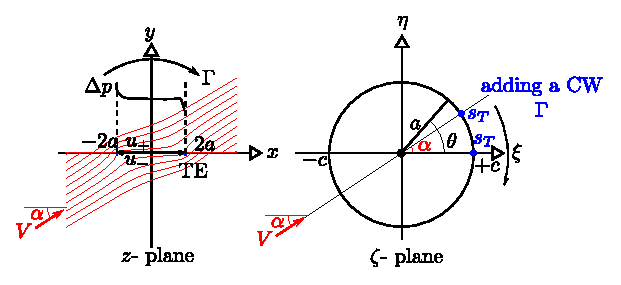
\includegraphics[scale=1.8]{figure/chapter5/5-1-38.eps}
%\caption{\label{fig:blue_rectangle} Rectangle}
\end{figure}
\[
F(\zeta) = V\left(\zeta e^{-i\alpha} + \frac{a^2}{\zeta}e^{i\alpha}\right) + \frac{i\Gamma}{2\pi}\ln\zeta
\]
\[
\frac{dF}{dz} = \frac{dF}{d\zeta}/\frac{dz}{d\zeta} \equiv\text{ finite at TE }(\zeta = a)
\]
i.e.
\begin{align*}
\left.\frac{dF}{d\zeta}\right|_{\zeta = a} = 0, &&\frac{dF}{d\zeta} = Ve^{-i\alpha} - V\frac{a^2e^{i\alpha}}{\zeta^2} + \frac{i\Gamma}{2\pi}\frac{1}{\zeta}
\end{align*}
\[
\left.\frac{dF}{d\zeta}\right|_{\zeta = a} = 0\Longrightarrow Ve^{-i\alpha} - Ve^{i\alpha} + \frac{i\Gamma}{2\pi a} = 0
\]
\[
\Longrightarrow\boxed{\Gamma = 4\pi Va\sin\alpha}
\]
Velocity on the plate:
\begin{align*}
\left.\frac{dF}{d\zeta}\right|_{\text{plate}} \equiv\left.\frac{dF}{d\zeta}\right|_{\zeta = ae^{i\theta}}
&= Ve^{-i\alpha} - Ve^{i\left(\alpha-2\theta\right)} + \frac{i\Gamma}{2\pi a}e^{-i\theta} = \cdots \\
&= Ve^{-i\theta}\left[e^{-i\left(\alpha-\theta\right)} - e^{i\left(\alpha-\theta\right)} + i2\sin\alpha\right] \\
&= 2iVe^{-i\theta}\left[\sin\alpha-\sin\left(\alpha-\theta\right)\right]
\end{align*}
\[
\left.\frac{dz}{d\zeta}\right|_{\text{plate}}\equiv\left.\frac{dz}{d\zeta}\right|_{\zeta = ae^{i\theta}} = 1-e^{-2i\theta} = e^{-i\theta}\left[e^{i\theta}-e^{-i\theta}\right] = 2i\sin\theta e^{-i\theta}
\]
\begin{align*}
\Longrightarrow
\left.\frac{dF}{dz}\right|_{\text{plate}} = \left.\frac{dF}{d\zeta}/\frac{dz}{d\zeta}\right|_{\text{plate}}
&= \frac{2iVe^{-i\theta}\left[\sin\alpha-\sin\left(\alpha-\theta\right)\right]}{2i\sin\theta e^{-i\theta}} \\
&= \frac{V\left[\sin\alpha-\sin\alpha\cos\theta+\cos\alpha\sin\theta\right]}{\sin\theta}\\ 
&= \cdots \\
&= V\cos\alpha\left(1+\tan\alpha\frac{1-\cos\theta}{\sin\theta}\right)\equiv \left.u-iv\right|_{\text{plate}}
\end{align*}
on the plate
\[
\left\{
\begin{aligned}
u &= V\cos\alpha\left(1+\tan\alpha\frac{1-\cos\theta}{\sin\theta}\right), 0<\theta\leq \pi\colon\text{upper surface of plate} \\
v &= 0,\pi<\theta\leq 2\pi\colon\text{lower surface of plate}
\end{aligned}
\right.
\]
From Bernoulli's equation
\[
p_+ + \frac{\rho}{2}u_+^2 = p_- + \frac{\rho}{2}u_-^2
\]
\begin{align*}
\Delta p
&\equiv p_- - p_+ = \frac{\rho}{2}\left(u_+^2 - u_-^2\right) \\
&= \frac{\rho}{2}V^2\cos^2\alpha\left[\left(1 + \tan\alpha\frac{1-\cos\theta}{\sin\theta}\right)^2 - \left(1 - \tan\alpha\frac{1-\cos\theta}{\sin\theta}\right)^2\right] \\
&= \rho V^2\sin\alpha\frac{1-\cos\theta}{\sin\theta}, \text{ $0\leq\theta\leq\pi$}
\end{align*}
Lift force $Y$
\begin{align*}
Y 
&= \int_{-2a}^{2a}\Delta p dx \vc{=}{\footnotemark}{} \int_{\theta = \pi}^{\theta = 0}\Delta p d\left(2a\cos\theta\right) = 2a\int_0^{\pi}\Delta p \sin\theta d\theta  \\
&= 2\rho V^2a\sin 2\alpha\int_0^{\pi}\left(1-\cos\theta\right)d\theta = 2\pi\rho V^2a\sin 2\alpha
\end{align*}
\footnotetext{From J-T $\displaystyle z = \zeta + \frac{a^2}{\zeta},\zeta = ae^{i\theta}$, $z=a^{i\theta} + ae^{-i\theta} = 2a\cos\theta = x+iy\Longrightarrow
\left\{
\begin{aligned}
x &= 2a\cos\theta \\
y &= 0
\end{aligned}
\right.
$}
or from Kutta-Joukowski Theorem
\begin{align*}
X - iY = -i\rho Ve^{-i\alpha}\Gamma, &&\text{ Here }\Gamma = 4\pi Va\sin\alpha
\end{align*}
\[
\therefore X-iY = -4\pi\rho V^2a\sin^2\alpha-i4\pi\rho V^2a\sin\alpha\cos\alpha
\]
\[
\Longrightarrow
\left\{
\begin{aligned}
X &= -4\pi\rho V^2a\sin^2\alpha\neq 0 \\
Y &= 4\pi \rho V^2a\sin\alpha\cos\alpha
\end{aligned}
\right.
\]
\end{example}
\subsection{Schwarz-Christoffel Transformation}
\begin{figure}[H]
\centering
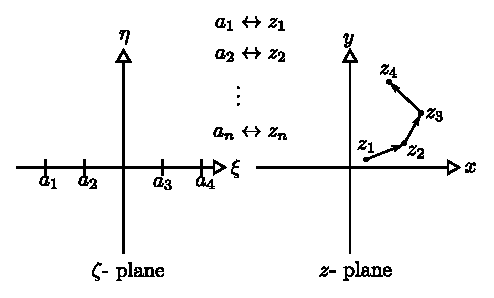
\includegraphics[scale=1.8]{figure/chapter5/5-1-39.eps}
%\caption{\label{fig:blue_rectangle} Rectangle}
\end{figure}
At critical point of transformation
\[
\text{A smooth curve}\Longleftrightarrow\text{A corner}
\]
The transformation has the form
\begin{equation}
\frac{dz}{d\zeta} = K\left(\zeta-a_1\right)^{k_1-1}\left(\zeta-a_2\right)^{k_2-1}\cdots\left(\zeta-a_N\right)^{k_N-1} \text{ (S-C T)}
\label{eq: 5-3-60}
\end{equation}
where $a_1,a_2,\cdots a_N$ are real numbers, $k_1,k_2,\cdots k_N$ are real numbers, and $K$ is a complex number.
\begin{itemize}
\item General properties and rules of S-C T
\begin{figure}[H]
\centering
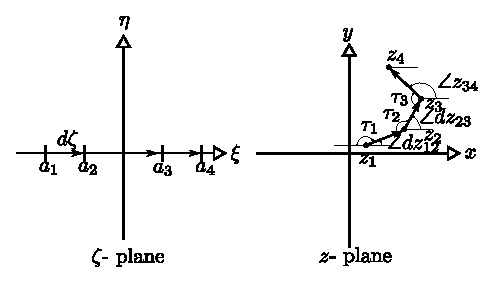
\includegraphics[scale=1.8]{figure/chapter5/5-1-40.eps}
%\caption{\label{fig:blue_rectangle} Rectangle}
\end{figure}
S-C T\\
\[
\frac{dz}{d\zeta} = K\left(\zeta - a_1\right)^{k_1-1}\left(\zeta - a_2\right)^{k_2-1}\cdots
\]
\begin{equation}
\begin{aligned}
\Longrightarrow\angle dz - \angle d\zeta 
&= \angle K + \left(k_1-1\right)\angle \left(\zeta-a_1\right) \\ 
&+ \left(k_2-1\right)\angle \left(\zeta-a_2\right) + \cdots
\end{aligned}
\tag{$\ast$}
\label{eq: 5-3-5-*}
\end{equation}
\begin{enumerate}[label = \protect\circled{\arabic*}]
\item $\zeta$ is between $\zeta = a_1$ and $\zeta = a_2$\\
\begin{align*}
\Longrightarrow \angle d\zeta =  0&& \text{ and } && \angle\left(\zeta-a_1\right) = 0,\angle\left(\zeta-a_2\right)=\angle\left(\zeta-a_3\right) =\cdots = \pi
\end{align*}
Between $z_1$ and $z_2$, from \eqref{eq: 5-3-5-*}
\[
\Longrightarrow
\angle dz_{12} - 0 = \angle K + \pi\sum_{i=2}^N\left(k_i-1\right) = \text{ constant}
\]
So segment from $z_1$ and $z_2$ is a \emph{straight line}.
\item $\zeta$ is between $\zeta = a_2$ and $\zeta = a_3$\\
\[
\angle\left(\zeta-a_1\right)=\angle\left(\zeta-a_2\right)=0
\]
\[
\angle\left(\zeta-a_3\right) = \angle\left(\zeta-a_4\right) = \cdots = \pi
\]
\begin{align*}
\eqref{eq: 5-3-5-*}\Longrightarrow
\angle dz_{23} - 0
&= \angle K + \pi\sum_{i=3}^N\left(k_i-1\right) = \text{ constant} \\
&= \angle K + \pi\sum_{i=2}^N\left(k_i-1\right) - \pi\left(k_2-1\right) \\
&= \angle dz_{12} - \pi\left(k_2-1\right)
\end{align*}
\[
\Longrightarrow\angle dz_{23} - \angle dz_{12} = -\pi\left(k_2-1\right) = \pi -\tau_2
\]
\[
\Longrightarrow\boxed{k_2=\frac{\tau_2}{\pi}}
\]
\begin{center}
\begin{tikzpicture}
\coordinate (O) at (0,0);
\node[below left] at (O) {$O$};
\fill[color=black] (O) circle[radius=2pt] ;
\coordinate (z2) at (3,2);
\node[below right] at (z2) {$z_2$};
\fill[color=black] (z2) circle[radius=2pt] ;
\coordinate (z3) at (1,5);
\node[below left] at (z3) {$z_3$};
\fill[color=black] (z3) circle[radius=2pt] ;
\draw [color=black,-{Latex[length=3mm]}, rotate=0] (O) -- (z2) ;
\draw [color=black,-{Latex[length=3mm]}, rotate=0] (z2) -- (z3) ;
\coordinate (z2dash) at (4.5,3);
\draw [dashed] (z2) -- (z2dash) ;
\draw pic["$dz_{23}-dz_{12}=-\pi\left(k_2-1\right)=\pi - \tau_2$", draw=red, text=red, ->, angle eccentricity=1.4, angle radius=1.0cm] {angle=z2dash--z2--z3};
\draw pic["$\tau_2$", draw=red, text=red, <-, angle eccentricity=1.4, angle radius=0.7cm] {angle=z3--z2--O};
\end{tikzpicture}
\end{center}
\begin{example}{For a Pentagon, the S-C T is }
\begin{figure}[H]
\centering
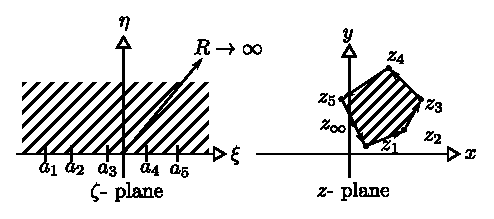
\includegraphics[scale=1.8]{figure/chapter5/5-1-41.eps}
%\caption{\label{fig:blue_rectangle} Rectangle}
\end{figure}
\[
\frac{dz}{d\zeta} = K\left(\zeta-a_1\right)^{k_1-1}\left(\zeta-a_2\right)^{k_2-1}\cdots\left(\zeta-a_5\right)^{k_5-1}
\]
The points $\infty$ on $\zeta$- plane, say $\zeta = Re^{i\varphi}$ ($R\to\infty$), will map to a \emph{point} $z_\infty$ on $z$- plane. \\
From \eqref{eq: 5-3-60}
\begin{align*}
\frac{dz}{d\zeta} 
&= K\zeta^{k_1-1}\zeta^{k_2-1}\cdots\zeta^{k_N-1} \\
&\left(1-\frac{a_1}{\zeta}\right)^{k_1-1}\left(1-\frac{a_2}{\zeta}\right)^{k_2-1}\cdots\left(1-\frac{a_N}{\zeta}\right)^{k_N-1}\\
&= K\zeta^{\sum_{i=1}^N\left(k_i-1\right)}\left[1-\frac{\sum_{i=1}^N\left(k_i-1\right)}{\zeta}+\mathcal{O}(\frac{1}{\zeta^2})\right]
\end{align*}
Integral $\Longrightarrow$
\[
z = K\frac{\zeta^{1+\sum_{i=1}^N\left(k_i-1\right)}}{1 + \sum_{i=1}^N\left(k_i-1\right)}\left[1+\mathcal{O}(\frac{1}{\zeta})\right] + C
\]
but 
\begin{align*}
1 + \sum_{i=1}^N\left(k_i-1\right)
&= 1 + \sum_{i=1}^N\left(\frac{\tau_i}{\pi} - 1\right) = 1-N+\sum_{i=1}^N\frac{\tau_i}{\pi} \\
&= 1-N+\left[\frac{\left(N-2\right)\pi}{\pi}\right] = -1
\end{align*}
\begin{equation}
\therefore z = K\left(-\frac{1}{\zeta}\right)\left[1 + \mathcal{O}(\frac{1}{\zeta})\right] + C
\label{eq: 5-3-62}
\end{equation}
hence as $\zeta\to\infty$, $z\to C$
\end{example}
\item The action of $K$ in $\displaystyle\frac{dz}{d\zeta}$ is to magnify $K=\sigma e^{i\psi}$ and rotate the polygon on $z$- plane
\end{enumerate}
\item Some considerations in constructing the S-C T\\
Q: Given $z_1,z_2,\cdots, z_N$, (and hence $\tau_1,\tau_2,\cdots,\tau_N$), how to choose $a_1,a_2,\cdots,a_N$?
\end{itemize}
\begin{note}\mbox{}\\
integrate $\eqref{eq: 5-3-60}$
\begin{equation}
\Longrightarrow z = K\int_{a_1}^{\zeta}\left(\zeta-a_1\right)^{k_1-1}\left(\zeta-a_2\right)^{k_2-1}\cdots\left(\zeta-a_N\right)^{k_N-1}d\zeta + z_1
\label{eq: 5-3-63}
\end{equation}
\underline{Observations:}
\begin{enumerate}[label = \protect\circled{\arabic*}]
\item $a_1$ is arbitrary
\item Having chosen $a_1$, \eqref{eq: 5-3-63} becomes
\begin{align*}
z_2 - z_1
&= K\int_{a_1}^{a_2}\left(\zeta-a_1\right)^{k_1-1}\left(\zeta-a_2\right)^{k_2-1}\cdots\left(\zeta-a_N\right)^{k_N-1}d\zeta \\
&= KF_2\left(a_2,a_3,\cdots,a_N\right)\\
z_3 - z_2
&= K\int_{a_2}^{a_3}\left(\zeta-a_1\right)^{k_1-1}\left(\zeta-a_2\right)^{k_2-1}\cdots\left(\zeta-a_N\right)^{k_N-1}d\zeta \\
&= KF_3\left(a_2,a_3,\cdots,a_N\right) \\
&\vdots \\
z_N - z_{N-1}
&= K\int_{a_{N-1}}^{a_N}\left(\zeta-a_1\right)^{k_1-1}\left(\zeta-a_2\right)^{k_2-1}\cdots\left(\zeta-a_N\right)^{k_N-1}d\zeta \\
&= KF_N\left(a_2,a_3,\cdots,a_N\right)
\end{align*}
where are $N-1$ constraints and $N-1$ equations (redundant: $z_1-z_N$)\\
but have $N$ unknowns, $a_2,a_3,\cdots,a_N,N$ hence another, say $a_2$, can be chosen arbitrary. Only $N-2$ constraints, not $N-1$, hence still another, say $a_3$, can be chosen arbitrary. 
\begin{conclusion}
Among $a_1$ and $a_N$ can arbitrary choose 3 of them (say $a_1,a_2,a_3$). Since arbitrary, for convenience, can take on of then, say $\boxed{a_1}\to -\infty$
\begin{align*}
\frac{dz}{d\zeta}
&= K\left(-a\right)^{k_1-1}\cancel{\left(1-\frac{\zeta}{a_1}\right)^{k_1-1}}\left(\zeta-a_2\right)^{k_2-1}\cdots \\
&= K\left(-a\right)^{k_1-1}\left(\zeta-a_2\right)^{k_2-1}\left(\zeta-a_3\right)^{k_3-1}\cdots \\
&= K'\left(\zeta-a_2\right)^{k_2-1}\left(\zeta-a_3\right)^{k_3-1}\cdots
\end{align*}
\end{conclusion}
\end{enumerate}
\end{note}